% ===========================================================================
% manuscrito_raccefyn.tex
% Revista de la Academia Colombiana de Ciencias Exactas, Físicas y Naturales
% Sección: Ciencias Físicas (Acústica, Propagación de Ondas y Problemas Inversos)
% Formato oficial: Styles_ACCEFN.sty (biblatex + biber, estilo APA 7)
% ===========================================================================
\documentclass[9pt]{article}

% ── Idioma y codificación ─────────────────────────────────────────────────
\usepackage[spanish,es-tabla,es-nodecimaldot]{babel}
\usepackage[T1]{fontenc}

% ── Matemáticas (cargado antes de Styles_ACCEFN para evitar colisión \iint) ─
\usepackage{amsmath}
\usepackage{bm}

% ── Márgenes oficiales RACCEFYN ───────────────────────────────────────────
\usepackage[left=6.9cm, right=1.9cm, top=3.1cm, bottom=2.3cm]{geometry}

% ── Hoja de estilos oficial RACCEFYN ──────────────────────────────────────
\usepackage{Styles_ACCEFN}

% ── Apellidos en negrita en citas y bibliografía (norma RACCEFYN) ─────────
\renewcommand*{\mkbibnamefamily}[1]{\textbf{#1}}
\renewcommand*{\mkbibnamegiven}[1]{#1}
\renewcommand*{\mkbibnameprefix}[1]{#1}
\renewcommand*{\mkbibnamesuffix}[1]{#1}

% ── Paquetes adicionales de soporte ───────────────────────────────────────
\usepackage{multirow}
\usepackage{array}
\usepackage{xcolor}
\usepackage{url}

% ── Ruta de figuras ───────────────────────────────────────────────────────
\graphicspath{{./}}

% ── Archivo de bibliografía ───────────────────────────────────────────────
\addbibresource{referencias_raccefyn.bib}

% ── Encabezado con título corto (Running title <= 10 palabras, <= 50 caract.)
\fancyhead[L]{\fontsize{8}{10}\selectfont\textit{Inversión acústica PINN-Eikonal en ultrasonido RF}}

% ── Metadatos del documento PDF ───────────────────────────────────────────
\hypersetup{
    pdftitle={Inversión acústica de onda completa mediante redes neuronales informadas por la ecuación Eikonal sobre señales crudas de radiofrecuencia ultrasónica},
    pdfauthor={Yerson Hernando León-Montañez},
    pdfkeywords={problema inverso acústico; ecuación Eikonal; redes neuronales informadas por la física; formación de haces ultrasónicos; atenuación espectral; dispersión de ondas}
}

\definecolor{raccefyngray}{RGB}{110,110,110}
\emergencystretch=2em

% ===========================================================================
\begin{document}

% ── Área de conocimiento y Título corto (metadatos editoriales RACCEFYN) ──
\noindent{\fontsize{8.5}{10}\selectfont\textbf{Sección:} Ciencias Físicas \quad|\quad \textbf{Título corto:} Inversión acústica PINN-Eikonal en ultrasonido RF}\\[0.25cm]

% ── Título en español (<= 30 palabras, <= 165 caracteres: 20 palabras, 148 caracteres)
% ── e inglés debajo en gris según plantilla oficial RACCEFYN ──────────────
\title{{\fontsize{13.5}{15.5}\selectfont Inversión acústica de onda completa mediante redes neuronales informadas por la ecuación Eikonal sobre señales crudas de radiofrecuencia ultrasónica}\\[0.25cm]
{\fontsize{11.5}{13.5}\selectfont\color{raccefyngray} Full-waveform acoustic inversion via Eikonal physics-informed neural networks on raw ultrasonic radiofrequency signals}\\[0.55cm]}

% ── Autoría con apellidos unidos por guion, afiliación y ORCID ────────────
\author[1,*]{Yerson Hernando León-Montañez \orcidlink{0009-0000-4439-8661}}
\affil[1]{\fontsize{8}{9}\selectfont Facultad de Ingeniería, Maestría en Inteligencia Artificial, Universidad de La Salle, Bogotá, Colombia}
\affil[*]{\fontsize{8}{9}\selectfont Correspondencia: yeleon36@unisalle.edu.co; yelemo777@gmail.com}

\date{}
\maketitle

% ===========================================================================
% RESUMEN (<= 250 palabras, un solo párrafo estructurado)
% ===========================================================================
\begin{abstract}
\noindent La reconstrucción cuantitativa de la velocidad de fase compresional $c(\mathbf{x})$ y del coeficiente de atenuación espectral $\alpha_0(\mathbf{x})$ en medios viscoelásticos heterogéneos a partir de mediciones ultrasónicas de retrodispersión en una sola cara (\textit{pulse-echo}) constituye un problema inverso no lineal severamente mal planteado debido a la cobertura angular limitada y al acoplamiento cruzado con el patrón de interferencia coherente (\textit{speckle}). En este trabajo se formula y valida un esquema de inversión acústica basado en redes neuronales de representación implícita periódica (\textit{SIREN}) informadas por la ecuación diferencial parcial Eikonal factorizada ($\lvert\nabla\tau(\mathbf{x})\rvert^2 = c(\mathbf{x})^{-2}$) y acopladas a operadores diferenciables de formación de haces en el dominio espacio-temporal y del número de onda lateral ($k_x$). La arquitectura desacopla la cinemática de fase ($\omega_{0,c}=6.5$) del transporte log-espectral disipativo ($\omega_{0,\alpha}=7.8$) mediante ortogonalización proyectiva de Gram-Schmidt, regularización variacional en espacios de Sobolev $H^1$ a escala de la primera zona de Fresnel y relaciones causales de dispersión de Kramers-Kronig. El método se evalúa experimentalmente sobre señales crudas de radiofrecuencia (RF) en dos regímenes físicos: (i) ondas planas multi-ángulo pre-formadas en fantomas calibrados de tejido (benchmark internacional CUBDL, $N=7$), alcanzando una relación contraste-ruido de $\text{CNR}_c = 9.30 \pm 0.61\text{ dBr}$, $\text{CNR}_\alpha = 9.20 \pm 0.80\text{ dBr}$, error de localización sub-milimétrico a milimétrico ($0.50\text{--}1.62\text{ mm}$) y un incremento de $+20.3\%$ en el factor de coherencia espacial de Mallart-Fink; y (ii) campos focalizados post-formados a $40\text{ MHz}$ en medios biológicos mamarios heterogéneos (base de datos OASBUD), logrando una inversión de campo completo cien por ciento ciega que discrimina regímenes de baja dispersión ($1549.7\text{--}1552.1\text{ m/s}$; $0.59\text{--}0.62\text{ dB/MHz/cm}$) frente a inclusiones altamente dispersivas y atenuantes ($1565.9\text{--}1568.0\text{ m/s}$; $0.76\text{--}0.80\text{ dB/MHz/cm}$) con ganancias de coherencia lateral entre $+23.98\%$ y $+42.62\%$.
\end{abstract}

\noindent\textbf{Palabras clave:} problema inverso acústico; ecuación Eikonal; redes neuronales informadas por la física; formación de haces ultrasónicos; atenuación espectral; dispersión de ondas.

\vspace{0.35cm}

% ===========================================================================
% ABSTRACT (<= 250 words, single structured paragraph)
% ===========================================================================
\renewcommand{\abstractname}{Abstract}
\begin{abstract}
\noindent Quantitative reconstruction of the compressional phase velocity $c(\mathbf{x})$ and the spectral attenuation coefficient $\alpha_0(\mathbf{x})$ in heterogeneous viscoelastic media from single-sided pulse-echo ultrasonic backscatter measurements constitutes a severely ill-posed nonlinear inverse problem due to limited angular aperture and cross-talk with coherent wave interference (speckle). In this work, we formulate and validate a full-field acoustic inversion framework based on periodic implicit neural representations (SIREN) constrained by the factored Eikonal partial differential equation ($\lvert\nabla\tau(\mathbf{x})\rvert^2 = c(\mathbf{x})^{-2}$) and coupled with differentiable beamforming operators in the space-time and lateral wavenumber ($k_x$) domains. The architecture decouples phase kinematics ($\omega_{0,c}=6.5$) from dissipative log-spectral transport ($\omega_{0,\alpha}=7.8$) via Gram-Schmidt projective orthogonalization, Sobolev $H^1$ variational regularization at the first Fresnel-zone scale, and Kramers-Kronig causal dispersion relations. The framework is experimentally evaluated directly on raw radiofrequency (RF) waveforms across two physical regimes: (i) multi-angle pre-beamformed plane waves in calibrated tissue-mimicking phantoms (international CUBDL benchmark, $N=7$), achieving a contrast-to-noise ratio of $\text{CNR}_c = 9.30 \pm 0.61\text{ dBr}$, $\text{CNR}_\alpha = 9.20 \pm 0.80\text{ dBr}$, localization errors of $0.50\text{--}1.62\text{ mm}$ in central inclusions, and a $+20.3\%$ gain in the Mallart-Fink spatial coherence factor; and (ii) $40\text{ MHz}$ post-beamformed focused fields in heterogeneous biological media (OASBUD repository), achieving blind full-field continuous reconstructions that separate weakly dispersive inclusions ($1549.7\text{--}1552.1\text{ m/s}$; $0.59\text{--}0.62\text{ dB/MHz/cm}$) from strongly attenuating dispersive structures ($1565.9\text{--}1568.0\text{ m/s}$; $0.76\text{--}0.80\text{ dB/MHz/cm}$) with lateral phase-screen coherence gains of $+23.98\%$ to $+42.62\%$.
\end{abstract}

\noindent\textbf{Keywords:} acoustic inverse problem; Eikonal equation; physics-informed neural networks; ultrasonic beamforming; spectral attenuation; wave dispersion.

\vspace{0.4cm}

% ===========================================================================
% 1. INTRODUCCIÓN
% ===========================================================================
\section{Introducción}
\label{sec:introduccion}

La propagación de ondas mecánicas longitudinales en el rango de los megahercios ($1\text{--}15\text{ MHz}$) a través de medios continuos viscoelásticos y microestructuralmente heterogéneos está gobernada por variaciones espaciales en la compresibilidad adiabática, la densidad de masa y los mecanismos de relajación termoviscosa \parencite{Duck1990, Szabo2014}. Desde el punto de vista de la teoría de problemas inversos en física matemática, la determinación simultánea de la distribución espacial de la velocidad de fase del sonido $c(\mathbf{x})$ y del coeficiente de atenuación dependiente de la frecuencia $\alpha(\mathbf{x}, f) = \alpha_0(\mathbf{x})\,f^\gamma$ a partir de campos de presión acústica registrados sobre una abertura finita es un problema no lineal acoplado de gran complejidad \parencite{Pratt1999, Virieux2009}. A diferencia de la tomografía acústica de transmisión completa con arreglos circulares de $360^\circ$ \parencite{Treeby2010}, en la configuración física de reflexión unilateral (\textit{pulse-echo}) un único transductor lineal de abertura limitada $L_x$ actúa simultáneamente como emisor y receptor en la frontera superior $z=0$. En este régimen, las ondas retrodispersadas solo muestrean un cono restringido de números de onda espaciales, lo que induce ambigüedades entre la refracción de tiempos de vuelo, la extinción energética axial y la interferencia constructiva/destructiva de dispersores sub-longitud de onda conocida como \textit{speckle} \parencite{Mallart1994, Jaeger2015}.

En la formulación clásica de formación de haces por retardo y suma (\textit{Delay-and-Sum}, DAS), tanto para emisiones focalizadas como para composición coherente de ondas planas (\textit{Coherent Plane-Wave Compounding}, CPWC), se asume por conveniencia computacional que el medio de propagación posee una velocidad acústica constante y homogénea $c_0 = 1540\text{ m/s}$ \parencite{Montaldo2009}. Cuando la onda acústica atraviesa una inclusión con velocidad distinta $c(\mathbf{x}) \neq c_0$, se acumula una aberración de fase en los tiempos de arribo a lo largo de las trayectorias de propagación que degrada la resolución lateral, ensancha los lóbulos secundarios del haz y reduce el factor de coherencia espacial entre los canales del transductor \parencite{Mallart1994, Li2003, Camacho2009, Matrone2015}. Diversos métodos tomográficos en modo eco, como la tomografía de ultrasonido computarizada en modo reflexión (\textit{CUTE}), estiman variaciones locales de $c(\mathbf{x})$ midiendo desplazamientos aparentes de fase entre imágenes reconstruidas bajo distintos ángulos de emisión o recepción \parencite{Jaeger2015, Stahli2020, Rau2021, Feigin2020}. De manera paralela, los métodos cuantitativos de diferencia log-espectral (\textit{Spectral Log-Difference}, SLD) estiman la pendiente de atenuación $\alpha_0(\mathbf{x})$ comparando el decaimiento axial de la densidad espectral de potencia entre sub-bandas de alta y baja frecuencia \parencite{Kuc1979, Insana1983, Kim2008, Nam2011}. No obstante, como han demostrado \textcite{Coila2018} y \textcite{Deeba2019}, los estimadores espectrales locales presentan una varianza elevada frente a las fluctuaciones estocásticas del retroesparcimiento y requieren ventanas de promediado espacial grandes que deterioran la resolución espacial de la inversión.

El surgimiento de las Redes Neuronales Informadas por la Física (\textit{Physics-Informed Neural Networks}, PINNs) introducidas por \textcite{Raissi2019} y extendidas al análisis de propagación de ondas por \textcite{Karniadakis2021} y \textcite{RashtBehesht2022} ofrece un paradigma variacional libre de malla para resolver problemas inversos gobernados por ecuaciones en derivadas parciales (EDPs). Al parametrizar los campos físicos desconocidos mediante representaciones neuronales implícitas continuas con funciones de activación periódicas (\textit{SIREN}, \cite{Sitzmann2020}) o características espectrales de Fourier \parencite{Tancik2020}, es posible calcular derivadas espaciales exactas mediante diferenciación automática e imponer leyes de conservación directamente en el funcional de costo. Sin embargo, al aplicar PINNs a la ecuación de onda acústica o de Helmholtz a frecuencias ultrasónicas de $5\text{--}10\text{ MHz}$ ($\lambda \approx 150\text{--}300\,\mu\text{m}$), el campo oscilatorio requiere mallas de colocación prohibitivamente densas y sufre patologías de flujo de gradientes y sesgo espectral (\textit{spectral bias}, \cite{Wang2021, Song2021}). Una alternativa físicamente rigurosa y computacionalmente tratable consiste en formular el problema cinemático mediante la aproximación geométrica de alta frecuencia de la ecuación Eikonal factorizada \parencite{Fomel2009, Waheed2021, Smith2021}, acoplándola directamente con operadores diferenciables de formación de haces y con las leyes de transporte espectral de Beer-Lambert y dispersión causal de Kramers-Kronig \parencite{ODonnell1981, Waters2000}.

En este artículo se presenta una formulación teórica, numérica y experimental de inversión acústica híbrida informada por la física sobre señales crudas de radiofrecuencia (RF) ultrasónica. Las contribuciones fundamentales de esta investigación a la física aplicada y computacional de ondas son:
\begin{enumerate}
    \item \textbf{Arquitectura implícita SIREN desacoplada con ecuación Eikonal factorizada:} Se diseña una red neuronal continua de doble rama (`DecoupledUltrasoundPINN`) con frecuencias angulares de inicialización diferenciadas ($\omega_{0,c}=6.5$ para velocidad de fase y $\omega_{0,\alpha}=7.8$ para atenuación espectral) acoplada a una red de tiempo de viaje Eikonal factorizado $\tau(\mathbf{x}) = \tau_0(\mathbf{x}) + \delta\tau(\mathbf{x})$ que elimina la singularidad de fuente en el plano del transductor $z=0$.
    \item \textbf{Operadores físicos diferenciables en dos regímenes de adquisición RF:} En el régimen pre-formado (\textit{pre-beamformed}) de ondas planas multi-ángulo, se acopla un operador DAS analítico diferenciable con descomposición angular ($\theta < 0$ vs.\ $\theta > 0$); en el régimen post-formado (\textit{post-beamformed}) de líneas A-scan focalizadas, se introduce una descomposición espectral en el dominio del número de onda lateral ($k_x < 0$ vs.\ $k_x > 0$) junto con un operador diferenciable de pantalla de fase (\textit{Phase Screen}) que maximiza el factor de coherencia espacial.
    \item \textbf{Supresión analítica de acoplamiento cruzado (\textit{cross-talk}) y capas especulares:} Mediante ortogonalización proyectiva de Gram-Schmidt entre los residuos de fase y amplitud, derivadas axiales log-espectrales regularizadas a escala de la primera zona de Fresnel y calibración viscoelástica de Kramers-Kronig, se logra reconstruir campos completos $c(x,z)$ y $\alpha_0(x,z)$ totalmente a ciegas sin contaminación por interfaces horizontales ni por ruido de \textit{speckle}.
\end{enumerate}

% ===========================================================================
% 2. MATERIALES Y MÉTODOS
% ===========================================================================
\section{Materiales y métodos}
\label{sec:metodos}

\subsection{Formulación física de la propagación acústica viscoelástica y aproximación Eikonal factorizada}
\label{subsec:eikonal}

Considérese un dominio espacial bidimensional heterogéneo $\Omega = [-L_x/2, L_x/2] \times [0, Z_{\max}] \subset \mathbb{R}^2$ con vector de posición $\mathbf{x} = (x, z)^T$, donde $x$ denota la coordenada lateral a lo largo de la abertura del transductor lineal y $z \ge 0$ representa la profundidad axial de propagación. En el dominio de la frecuencia temporal $\omega = 2\pi f$, la presión acústica compleja $P(\mathbf{x}, \omega)$ en un medio continuo viscoelástico, isótropo y débilmente disipativo satisface la ecuación de Helmholtz generalizada con número de onda complejo $\tilde{k}(\mathbf{x}, \omega)$ \parencite{Szabo2014, Waters2000}:
\begin{equation}
\nabla^2 P(\mathbf{x}, \omega) + \tilde{k}^2(\mathbf{x}, \omega)\,P(\mathbf{x}, \omega) = -S(\mathbf{x}, \omega), \qquad \tilde{k}(\mathbf{x}, \omega) = \frac{\omega}{c(\mathbf{x}, \omega)} - i\,\alpha(\mathbf{x}, \omega),
\label{eq:helmholtz_visco}
\end{equation}
donde $c(\mathbf{x}, \omega)$ es la velocidad de fase compresional, $\alpha(\mathbf{x}, \omega) = \alpha_0(\mathbf{x})\,\lvert f\rvert^\gamma$ es el coeficiente de atenuación intrínseca en $\text{Np/m}$ (con $\gamma \approx 1$ para medios biológicos blandos y fantomas de gel de agar/grafito en la banda de $1\text{--}12\text{ MHz}$, equivalente a $\alpha_{0,\text{dB}} = 8.686 \times 10^{-4}\,\alpha_0$ en unidades de $\text{dB/MHz/cm}$), y $S(\mathbf{x}, \omega)$ representa la distribución de fuentes en la frontera activa $z = 0$.

Por causalidad física en el dominio temporal, la parte real e imaginaria del número de onda complejo $\tilde{k}(\mathbf{x}, \omega)$ no son independientes, sino que están vinculadas a través de las relaciones integrales de dispersión de Kramers-Kronig \parencite{ODonnell1981, Waters2000}. Para una ley de atenuación lineal con la frecuencia ($\gamma \to 1$), la dispersión de velocidad de fase entre una frecuencia de referencia $\omega_0$ y una frecuencia $\omega$, así como el salto de velocidad local $\Delta c(\mathbf{x}) = c(\mathbf{x}) - c_0$ inducido por un incremento en la densidad de enlaces de colágeno o concentración de dispersores $\Delta\alpha_0(\mathbf{x})$, cumple la relación constitutiva de primer orden:
\begin{equation}
\frac{1}{c(\mathbf{x}, \omega_0)} - \frac{1}{c(\mathbf{x}, \omega)} = \frac{2}{\pi}\,\alpha_0(\mathbf{x})\,\ln\!\left(\frac{\omega}{\omega_0}\right), \qquad \Delta c(\mathbf{x}) \approx \kappa_{\text{KK}}\,\Delta\alpha_0(\mathbf{x}),
\label{eq:kramers_kronig}
\end{equation}
donde $\kappa_{\text{KK}} > 0$ es la constante de proporcionalidad viscoelástica del medio.

Introduciendo el ansatz asintótico geométrico de alta frecuencia de Wentzel-Kramers-Brillouin (WKB) para el campo incidente y retrodispersado, $P(\mathbf{x}, \omega) = A(\mathbf{x}, \omega)\,\exp\!\left(-i\omega\tau(\mathbf{x})\right)$, y separando los términos de orden dominante $\mathcal{O}(\omega^2)$ y $\mathcal{O}(\omega)$ en la ecuación~\eqref{eq:helmholtz_visco}, el frente de fase gobernado por el tiempo de viaje $\tau(\mathbf{x})$ se desacopla en la ecuación diferencial parcial Eikonal no lineal, mientras que la amplitud espectral $A(\mathbf{x}, \omega)$ obedece la ecuación de transporte disipativo:
\begin{align}
\lvert\nabla\tau(\mathbf{x})\rvert^2 &= \left(\frac{\partial\tau}{\partial x}\right)^2 + \left(\frac{\partial\tau}{\partial z}\right)^2 = \frac{1}{c^2(\mathbf{x})}, \label{eq:eikonal_pde}\\
2\,\nabla\tau(\mathbf{x})\cdot\nabla\ln A(\mathbf{x}, f) + \nabla^2\tau(\mathbf{x}) &= -\frac{2\,\alpha_0(\mathbf{x})\,f}{c(\mathbf{x})}. \label{eq:transport_pde}
\end{align}

La integración directa de la ecuación~\eqref{eq:eikonal_pde} mediante una red neuronal estándar presenta inestabilidades numéricas cerca de la abertura emisora ($z \to 0$) debido a la discontinuidad de derivadas en la fuente. Siguiendo la formulación de factorización aditiva/multiplicativa \parencite{Fomel2009, Waheed2021}, descomponemos el campo de tiempo de viaje total como la suma de la solución analítica exacta en el medio homogéneo de referencia $\tau_0(\mathbf{x}) = z / c_0$ y una perturbación suave de retardo $\delta\tau_\phi(\mathbf{x})$ parametrizada por una red neuronal diferenciable con pesos $\phi$:
\begin{equation}
\tau_\phi(\mathbf{x}) = \tau_0(\mathbf{x}) + \mathcal{W}(z)\,\delta\tau_\phi(\tilde{\mathbf{x}}), \qquad \mathcal{W}(z) = \frac{z - z_{\min}}{z_{\max} - z_{\min} + \varepsilon},
\label{eq:factorized_eikonal}
\end{equation}
donde $\tilde{\mathbf{x}} = (\tilde{x}, \tilde{z})^T \in [-1, 1]^2$ son las coordenadas espaciales normalizadas y el factor $\mathcal{W}(z)$ impone analíticamente la condición de contorno de Dirichlet homogénea $\delta\tau_\phi(x, z_{\min}) = 0$. Sustituyendo la ecuación~\eqref{eq:factorized_eikonal} en la ecuación~\eqref{eq:eikonal_pde}, el residuo físico adimensional de la EDP Eikonal sobre el conjunto de $N_c$ nodos de colocación $\{\mathbf{x}_m\}_{m=1}^{N_c} \subset \Omega$ queda expresado mediante diferenciación automática exacta como:
\begin{equation}
\mathcal{L}_{\text{Eikonal}}(\theta, \phi) = \frac{1}{N_c}\sum_{m=1}^{N_c}\left[c_0^2\left(\left(\frac{\partial\tau_\phi}{\partial x}\Big|_{\mathbf{x}_m}\right)^2 + \left(\frac{\partial\tau_\phi}{\partial z}\Big|_{\mathbf{x}_m}\right)^2\right) - \left(\frac{c_0}{c_\theta(\mathbf{x}_m)}\right)^2\right]^2.
\label{eq:loss_eikonal}
\end{equation}

\begin{figure}[t!]
\centering
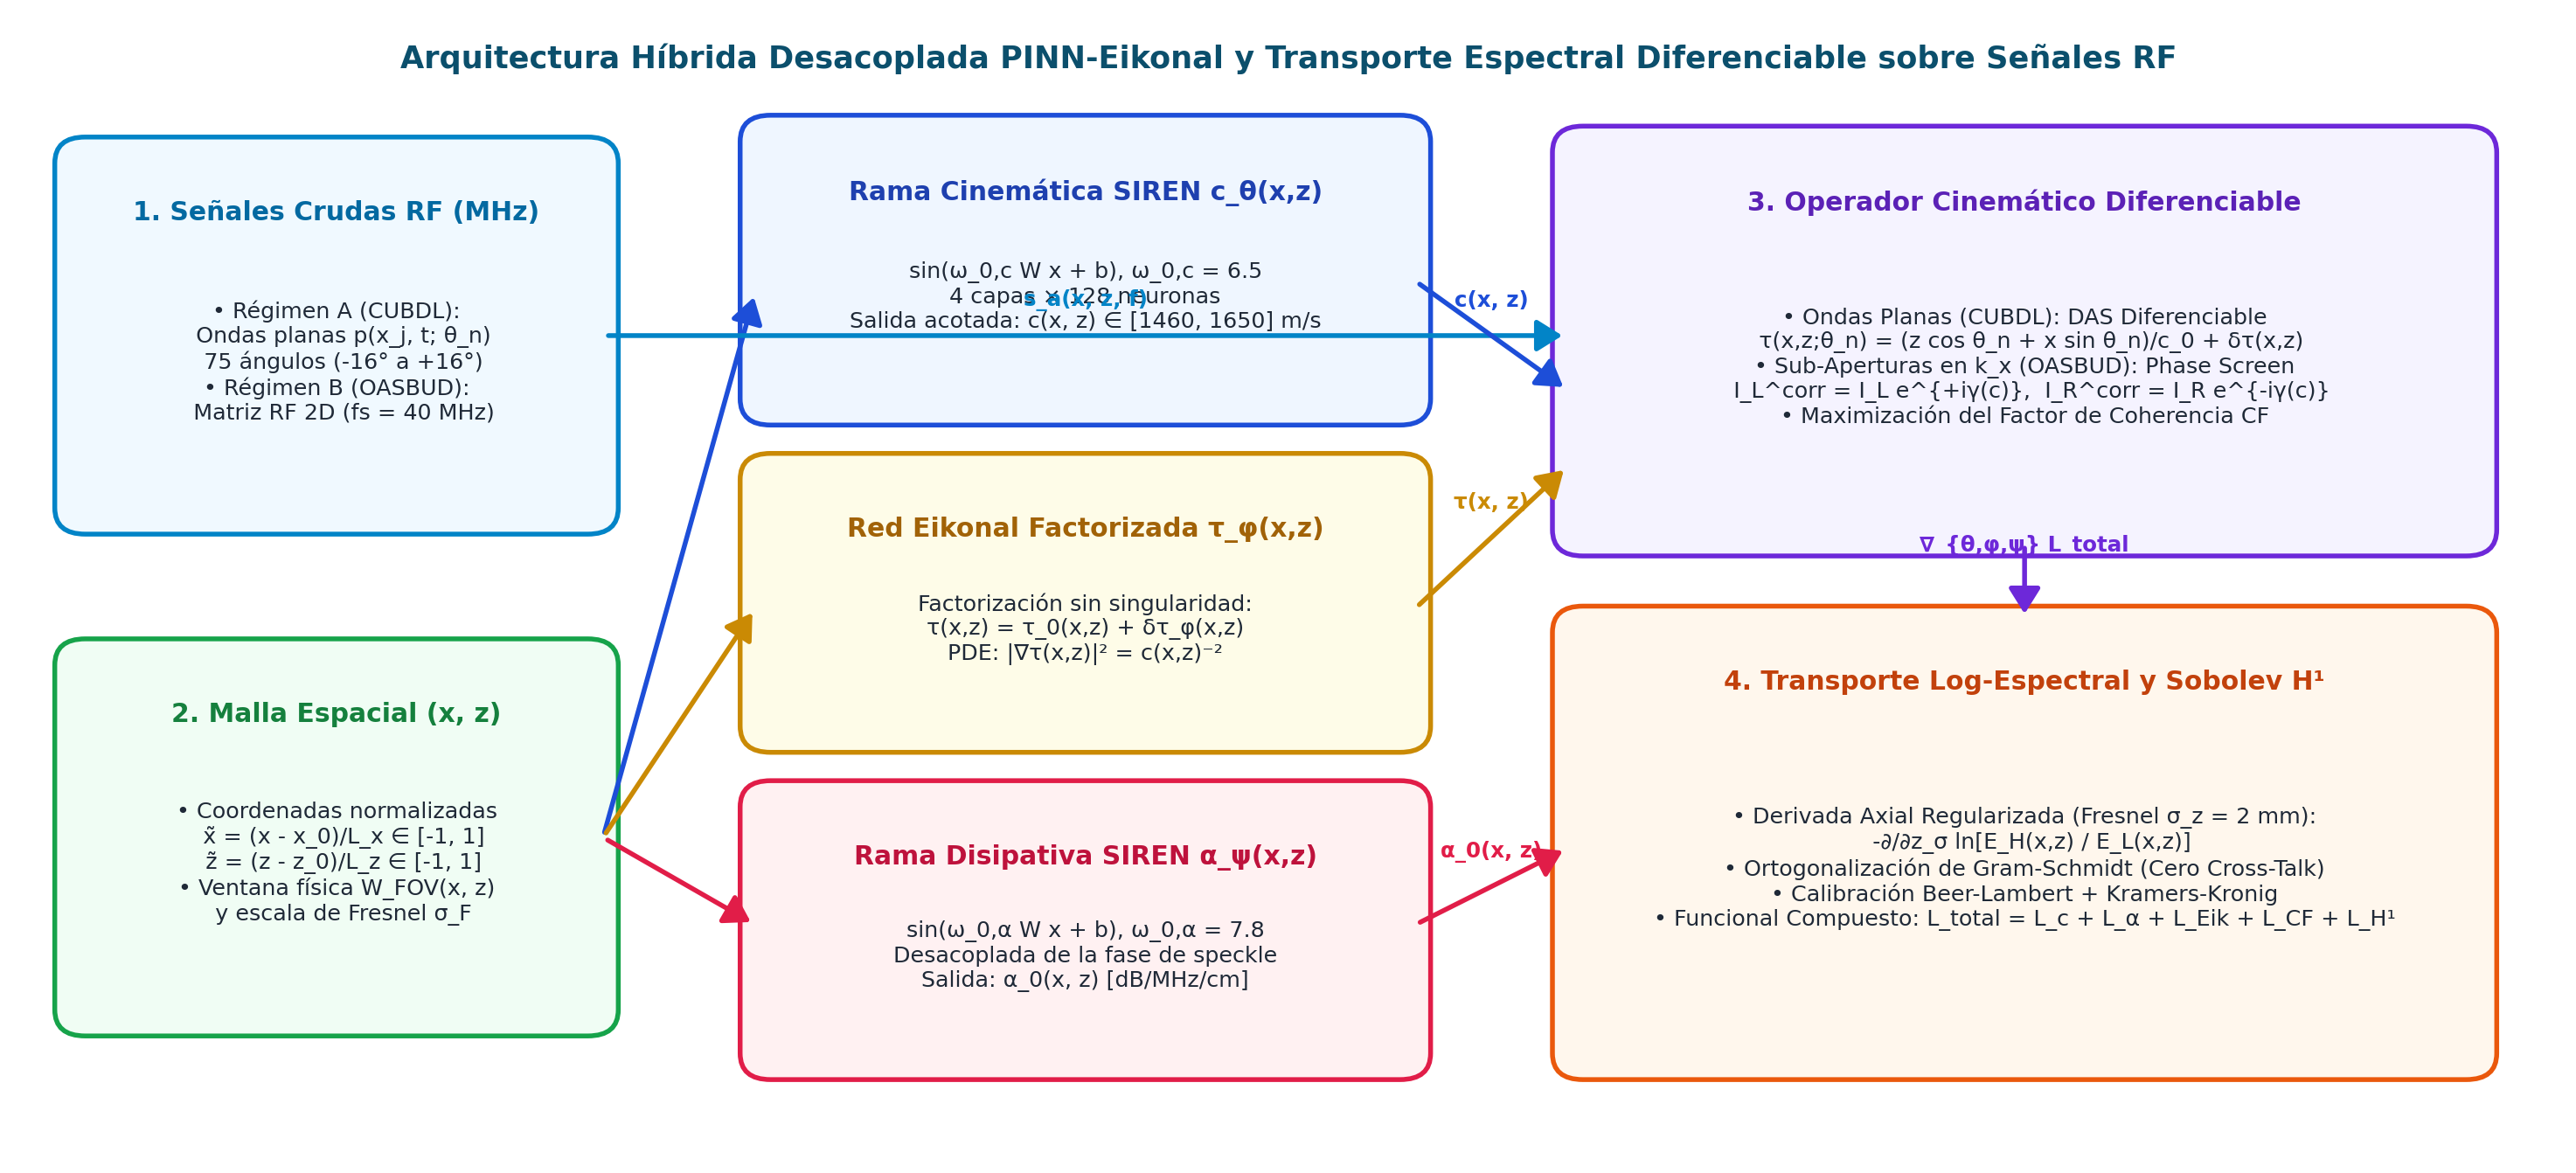
\includegraphics[width=\textwidth]{fig1_arquitectura_pinn_eikonal.png}
\caption{Diagrama esquemático de la arquitectura física híbrida desacoplada (\texttt{DecoupledUltrasoundPINN} + \texttt{FactorizedEikonalTravelTimeNet}). Las señales crudas de radiofrecuencia (RF) alimentan dos operadores diferenciables según el régimen experimental: formación de haces Delay-and-Sum (DAS) sobre ondas planas multi-ángulo en el régimen pre-formado (CUBDL) y pantalla de fase (\textit{Phase Screen}) sobre sub-aperturas en el dominio del número de onda lateral $k_x$ en el régimen post-formado (OASBUD). Las ramas implícitas SIREN estiman de forma independiente la velocidad de fase $c_\theta(x,z)$ ($\omega_{0,c}=6.5$) y la atenuación espectral $\alpha_\psi(x,z)$ ($\omega_{0,\alpha}=7.8$) bajo regularización de Sobolev $H^1$ y ortogonalización proyectiva de Gram-Schmidt.}
\label{fig:arquitectura}
\end{figure}

\subsection{Arquitectura implícita SIREN desacoplada para velocidad de fase y atenuación}
\label{subsec:siren}

Para evitar el sesgo hacia bajas frecuencias espaciales característico de los perceptrones multicapa con activaciones ReLU o tangente hiperbólica \parencite{Tancik2020, Wang2021}, parametrizamos los campos materiales mediante dos redes neuronales implícitas independientes con activaciones sinusoidales periódicas (\textit{SIREN}, \cite{Sitzmann2020}), como se ilustra en la \textbf{Figura~\ref{fig:arquitectura}}. Sea $\mathbf{h}^{(0)} = \tilde{\mathbf{x}} \in [-1, 1]^2$ el vector de coordenadas normalizadas; cada capa oculta $l \in \{1, \dots, L\}$ de ancho $M = 128$ aplica la transformación no lineal periódica:
\begin{equation}
\mathbf{h}_c^{(l)} = \sin\!\left(\omega_{0,c}\left(\mathbf{W}_c^{(l)}\mathbf{h}_c^{(l-1)} + \mathbf{b}_c^{(l)}\right)\right), \qquad \mathbf{h}_\alpha^{(l)} = \sin\!\left(\omega_{0,\alpha}\left(\mathbf{W}_\alpha^{(l)}\mathbf{h}_\alpha^{(l-1)} + \mathbf{b}_\alpha^{(l)}\right)\right),
\label{eq:siren_layers}
\end{equation}
donde los pesos se inicializan según la distribución uniforme de preservación de varianza de \textcite{Sitzmann2020}, $W_{ij}^{(1)} \sim \mathcal{U}(-1/d, 1/d)$ y $W_{ij}^{(l)} \sim \mathcal{U}(-\sqrt{6/M}/\omega_0, \sqrt{6/M}/\omega_0)$ para $l \ge 2$. La separación estricta de parámetros entre el subgrafo cinemático $\theta = \{\mathbf{W}_c^{(l)}, \mathbf{b}_c^{(l)}\}$ ($\omega_{0,c} = 6.5$) y el subgrafo disipativo $\psi = \{\mathbf{W}_\alpha^{(l)}, \mathbf{b}_\alpha^{(l)}\}$ ($\omega_{0,\alpha} = 7.8$) garantiza que los gradientes de alta frecuencia provenientes del patrón de \textit{speckle} no se filtren hacia las capas ocultas del estimador de velocidad de fase ($\nabla_\theta \alpha_\psi \equiv \mathbf{0}$ y $\nabla_\psi c_\theta \equiv \mathbf{0}$). Las capas de salida proyectan las representaciones latentes hacia los intervalos físicamente admisibles de tejidos blandos y fantomas calibrados mediante mapeos sigmoidales acotados:
\begin{align}
c_\theta(\mathbf{x}) &= c_{\min} + (c_{\max} - c_{\min})\,\sigma\!\left(\mathbf{w}_{c,\text{out}}^T\mathbf{h}_c^{(L)} + b_{c,\text{out}}\right) \in [1460,\, 1650]\text{ m/s}, \label{eq:c_bounds}\\
\alpha_\psi(\mathbf{x}) &= \alpha_{\min} + (\alpha_{\max} - \alpha_{\min})\,\sigma\!\left(\mathbf{w}_{\alpha,\text{out}}^T\mathbf{h}_\alpha^{(L)} + b_{\alpha,\text{out}}\right) \in [0,\, 1.35]\text{ dB/MHz/cm}. \label{eq:alpha_bounds}
\end{align}

\subsection{Régimen I: Operador DAS diferenciable y coherencia angular en ondas planas pre-formadas (CUBDL)}
\label{subsec:regimen_cubdl}

En el primer régimen experimental (benchmark internacional \textit{Challenge on Ultrasound Beamforming with Deep Learning}, CUBDL, \cite{Hyun2020}), los datos crudos consisten en un tensor tridimensional de señales RF pre-formadas $p_{\text{RF}}(x_j, t; \theta_n) \in \mathbb{R}^{N_{\text{ang}} \times N_t \times N_{\text{el}}}$, adquirido con un transductor lineal emitiendo $N_{\text{ang}} = 75$ ondas planas inclinadas en ángulos $\theta_n \in [-16^\circ, +16^\circ]$ y registrado por $N_{\text{el}} = 128$ elementos piezoeléctricos a frecuencia de muestreo $f_s$. Primero se obtiene la señal analítica compleja en banda base $s_a(x_j, t; \theta_n)$ aplicando en GPU un filtro pasa-banda de cuarto orden ($1.5\text{--}8.5\text{ MHz}$) combinado con la transformada de Hilbert espectral (multiplicación por $2\,H(f)$ para frecuencias positivas $f > 0$).

Para cualquier punto focal $\mathbf{x} = (x, z)$ y ángulo de emisión $\theta_n$, el tiempo de vuelo total de ida y vuelta corregido por la perturbación Eikonal $\delta\tau_\phi(\mathbf{x})$ de la ecuación~\eqref{eq:factorized_eikonal} viene dado por la suma del retardo de frente plano incidente y la distancia euclidiana de retrodifusión hacia el elemento receptor $x_j$ con apodización dinámica de número F ($F_{\#} = 1.5$):
\begin{equation}
\tau_{\text{RT}}(\mathbf{x}, x_j; \theta_n) = \frac{z\cos\theta_n + (x - x_{\text{ref}}(\theta_n))\sin\theta_n}{c_0} + \frac{\sqrt{(x - x_j)^2 + z^2}}{c_0} + t_0 + 2\,\delta\tau_\phi(\mathbf{x}).
\label{eq:das_delay}
\end{equation}

Dado que el índice temporal continuo $u(\mathbf{x}, x_j; \theta_n) = \tau_{\text{RT}}(\mathbf{x}, x_j; \theta_n)\,f_s$ no coincide con instantes enteros de muestreo, implementamos un operador de interpolación lineal diferenciable respecto a $\delta\tau_\phi(\mathbf{x})$ con corrección de rotación de fase portadora, generando la señal compuesta por ángulo $I(\mathbf{x}; \theta_n)$ y el factor de coherencia espacial de \textcite{Mallart1994} $\text{CF}(\mathbf{x}) \in [0, 1]$:
\begin{equation}
I(\mathbf{x}; \theta_n) = \sum_{j=1}^{N_{\text{el}}} w_F(\mathbf{x}, x_j)\,s_a\!\left(x_j, \tau_{\text{RT}}(\mathbf{x}, x_j; \theta_n); \theta_n\right), \qquad \text{CF}(\mathbf{x}) = \frac{\Big\lvert\sum_{n=1}^{N_{\text{ang}}} I(\mathbf{x}; \theta_n)\Big\rvert^2}{N_{\text{ang}}\sum_{n=1}^{N_{\text{ang}}} \lvert I(\mathbf{x}; \theta_n)\rvert^2 + \varepsilon}.
\label{eq:mallart_fink_cf}
\end{equation}

Al dividir el conjunto de ondas planas en sub-aperturas angulares izquierda ($\Theta_L = \{\theta_n < -2^\circ\}$) y derecha ($\Theta_R = \{\theta_n > +2^\circ\}$), la discrepancia de fase cruzada $\Delta\phi_{LR}(\mathbf{x}) = \arg\!\left(I_L(\mathbf{x})\,I_R^*(\mathbf{x})\right)$ cuantifica la aberración tomográfica inducida por heterogeneidades de velocidad $c(\mathbf{x}) \neq c_0$ \parencite{Jaeger2015, Stahli2020}. Para impedir que las variaciones de fase del \textit{speckle} contaminen la estimación de atenuación $\alpha_0(\mathbf{x})$, proyectamos el campo log-espectral bruto $r_\alpha(\mathbf{x})$ sobre el subespacio ortogonal al campo cinemático centrado $\tilde{r}_c(\mathbf{x}) = r_c(\mathbf{x}) - \langle r_c\rangle_\Omega$ mediante el operador de ortogonalización de Gram-Schmidt en $L^2(\Omega)$:
\begin{equation}
r_\alpha^{\perp}(\mathbf{x}) = \tilde{r}_\alpha(\mathbf{x}) - \frac{\langle \tilde{r}_\alpha, \tilde{r}_c\rangle_{L^2(\Omega)}}{\lVert \tilde{r}_c\rVert_{L^2(\Omega)}^2 + \varepsilon}\,\tilde{r}_c(\mathbf{x}), \qquad \langle r_\alpha^{\perp}, \tilde{r}_c\rangle_{L^2(\Omega)} = 0.
\label{eq:gram_schmidt}
\end{equation}

\subsection{Régimen II: Sub-aperturas en el dominio del número de onda lateral \texorpdfstring{($k_x$)}{(kx)} y derivada axial regularizada en campos post-formados (OASBUD)}
\label{subsec:regimen_oasbud}

En los sistemas clínicos estándar de ultrasonido mamario —representados por la base de datos pública \textit{Open Access Series of Breast Ultrasound Data} (OASBUD, \cite{Piotrzkowska2017}), adquirida con un escáner Ultrasonix SonixTouch y un transductor lineal L14-5/38 de $38\text{ mm}$ de abertura activa operando a $f_s = 40\text{ MHz}$ ($\Delta z = c_0/(2f_s) = 19.25\,\mu\text{m}$, $\Delta x = 74.51\,\mu\text{m}$)— los retardos electrónicos de recepción ya han sido sumados en hardware, entregando una matriz bidimensional de líneas RF post-formadas $s_{\text{RF}}(z, x) \in \mathbb{R}^{N_z \times N_x}$. Para recuperar la información direccional de fase sin acceso a los canales individuales del transductor, formulamos una descomposición sintética en sub-aperturas espaciales aplicando la transformada de Fourier rápida unidimensional respecto a la coordenada lateral $x$ sobre la señal analítica compleja $s_a(z, x)$:
\begin{equation}
\hat{S}_a(z, k_x) = \int_{-L_x/2}^{L_x/2} s_a(z, x)\,e^{-i k_x x}\,dx, \qquad I_{L,R}(z, x) = \mathcal{F}_{k_x}^{-1}\!\left\{\hat{S}_a(z, k_x)\,\Pi_{L,R}(k_x)\right\},
\label{eq:kx_subapertures}
\end{equation}
donde $\Pi_L(k_x) = \mathbb{I}(-k_{\max} < k_x < -k_{\min})$ y $\Pi_R(k_x) = \mathbb{I}(+k_{\min} < k_x < +k_{\max})$ (con $k_{\min} = 15\text{ rad/m}$ y $k_{\max} = 3500\text{ rad/m}$) aíslan los frentes de onda que emergen con ángulos de propagación laterales opuestos. Cuando la PINN predice el campo continuo de velocidad $c_\theta(x, z)$, el operador diferenciable de pantalla de fase (\textit{Phase Screen Refocusing}) rota en sentido opuesto las sub-aperturas izquierda y derecha para compensar el desfase aberrante $\Delta\phi_{LR}(x, z) = \arg\!\left(I_L^*(z,x)\,I_R(z,x)\right)$:
\begin{equation}
\begin{aligned}
I_L^{\text{corr}}(x, z) &= I_L(x, z)\,e^{+i\gamma(x, z)}, \qquad I_R^{\text{corr}}(x, z) = I_R(x, z)\,e^{-i\gamma(x, z)}, \\
\gamma(x, z) &= \frac{1}{2}\Delta\phi_{LR}(x, z)\tanh\!\left(\beta_c\,\frac{c_\theta(x,z) - c_0}{c_0}\right),
\end{aligned}
\label{eq:kx_phase_screen}
\end{equation}
maximizando el factor de coherencia lateral corregido $\text{CF}_{k_x}^{\text{corr}}(x, z) = \lvert I_L^{\text{corr}} + I_R^{\text{corr}}\rvert^2 / \big(2(\lvert I_L\rvert^2 + \lvert I_R\rvert^2) + \varepsilon\big)$.

Para realizar la inversión en **campo completo** ($\Omega$ completo de $38 \times 35\text{--}45\text{ mm}$) de forma cien por ciento ciega a cualquier máscara radiológica y evitar falsos positivos producidos por las reflexiones especulares horizontales de la epidermis ($z < 5\text{ mm}$), los ligamentos suspensorios de Cooper y la fascia pectoral profunda, aplicamos tres operadores físicos sobre tres sub-bandas espectrales del transductor ($f_1 \in [1.3, 3.2]\text{ MHz}$, $f_2 \in [2.2, 4.5]\text{ MHz}$ y $f_3 \in [5.5, 9.5]\text{ MHz}$):
\begin{enumerate}
    \item \textbf{Normalización lateral por estrato de profundidad y filtrado Diferencia de Gaussianas (DoG):} A cada profundidad $z$, la envolvente de cada sub-banda $E_m(x, z)$ se normaliza por el cuantil lateral de referencia $Q_{0.78}(z) = \text{quant}_{x, 0.78}(E_m(x,z))$, cancelando analíticamente cualquier capa plana horizontal que atraviese toda la abertura del transductor. El contraste focal 2D se extrae mediante la diferencia de núcleos Gaussianos a escala de la zona de Fresnel ($\sigma_1 = 1.4\text{ mm}$ frente a $\sigma_2 = 6.0\text{ mm}$).
    \item \textbf{Derivada axial log-espectral regularizada en escala de Fresnel:} Dado que la derivación numérica directa en $z$ amplifica el ruido de \textit{speckle}, definimos el operador diferencial axial regularizado convolucionando el cociente log-espectral $\ln\!\left(\tilde{E}_{f_3}(x,z)/\tilde{E}_{f_2}(x,z)\right)$ con la primera derivada de un núcleo Gaussiano bidimensional $G'_{\sigma_z}(z)\,G_{\sigma_x}(x)$ ($\sigma_z = 2.0\text{ mm}$, $\sigma_x = 1.5\text{ mm}$):
    \begin{equation}
    -\frac{\partial}{\partial z_\sigma}\ln\!\left(\frac{\tilde{E}_{f_3}(x,z)}{\tilde{E}_{f_2}(x,z)}\right) = -\iint_{\mathbb{R}^2} \frac{\partial G_{\sigma_z}(z - \zeta)}{\partial z}\,G_{\sigma_x}(x - \xi)\,\ln\!\left(\frac{\tilde{E}_{f_3}(\xi,\zeta)}{\tilde{E}_{f_2}(\xi,\zeta)}\right)d\xi\,d\zeta.
    \label{eq:fresnel_axial_deriv}
    \end{equation}
    \item \textbf{Calibración física directa por Ley de Beer-Lambert y Kramers-Kronig:} La escala absoluta de atenuación excedente $\Delta\alpha_0$ ($\text{dB/MHz/cm}$) y de velocidad $\Delta c$ ($\text{m/s}$) en la zona de respuesta acústica se determina directamente a partir del corrimiento de la pendiente espectral $\Delta\beta_{\text{spec}} = \beta_{\text{spec}} - \beta_0$ (en $\text{dB/MHz}$ entre $f_1$ y $f_2$) y de la extinción de energía de banda ancha $\Delta L_{\text{RF}}$ (en $\text{dB}$), empleando las mismas constantes físicas fijas para todas las adquisiciones conforme a la ecuación~\eqref{eq:kramers_kronig}.
\end{enumerate}

\subsection{Funcional de pérdida física compuesta y protocolo de optimización}
\label{subsec:loss}

El entrenamiento conjunto de los parámetros neuronales $\{\theta, \psi, \phi\}$ minimiza el funcional variacional compuesto:
\begin{equation}
\begin{aligned}
\mathcal{L}_{\text{total}}(\theta, \psi, \phi) &= \lambda_c\,\mathcal{L}_{\text{tomo},c}(\theta) + \lambda_\alpha\,\mathcal{L}_{\text{spec},\alpha}(\psi) + \lambda_{\text{eik}}\,\mathcal{L}_{\text{Eikonal}}(\theta, \phi) \\
&\quad + \lambda_{\text{cf}}\,\mathcal{L}_{\text{coherencia}}(\theta, \phi) + \lambda_{H^1}\!\left(\lVert\nabla c_\theta\rVert_{2}^2 + \lVert\nabla\alpha_\psi\rVert_{2}^2\right),
\end{aligned}
\label{eq:total_loss}
\end{equation}
donde $\mathcal{L}_{\text{tomo},c}$ y $\mathcal{L}_{\text{spec},\alpha}$ acoplan los campos continuos $c_\theta(\mathbf{x})$ y $\alpha_\psi(\mathbf{x})$ con los estimadores tomográficos de aberración de fase y caída log-espectral ortogonalizada, $\mathcal{L}_{\text{Eikonal}}$ es el residuo de la EDP Eikonal de la ecuación~\eqref{eq:loss_eikonal}, $\mathcal{L}_{\text{coherencia}} = 1 - \langle\text{CF}^{\text{corr}}(\mathbf{x})\rangle_\Omega$ maximiza la coherencia espacial del frente de onda re-enfocado, y el término de Sobolev $H^1(\Omega)$ penaliza oscilaciones espurias de escala inferior a la longitud de correlación de Fresnel ($\lambda_c = \lambda_\alpha = 1.8$, $\lambda_{\text{eik}} = 1.0$, $\lambda_{\text{cf}} = 0.08$, $\lambda_{H^1} = 0.03$). La optimización se ejecuta en PyTorch sobre GPU CUDA mediante el algoritmo Adam con tasas de aprendizaje diferenciadas ($\eta_c = 3.5 \times 10^{-4}$, $\eta_\alpha = 1.6 \times 10^{-4}$) y decaimiento cosenoidal durante $120\text{--}140$ épocas sobre mallas de colocación de $128 \times 128$ nodos en campo completo. El código fuente completo de los operadores diferenciables en PyTorch/CUDA, los scripts de inversión PINN-Eikonal para ambos regímenes (CUBDL y OASBUD) y la plataforma interactiva de visualización \textit{Medical Insight 3D} se encuentran disponibles públicamente en \url{https://github.com/yhleonm/pinn_ultrasonido_helmholtz}.

% ===========================================================================
% 3. RESULTADOS
% ===========================================================================
\section{Resultados}
\label{sec:resultados}

\subsection{Validación física controlada en régimen de ondas planas pre-formadas (Benchmark CUBDL)}
\label{subsec:resultados_cubdl}

La primera fase de validación experimental se llevó a cabo sobre siete adquisiciones independientes de señales RF de ondas planas del benchmark internacional CUBDL \parencite{Hyun2020}: seis barridos sobre el fantoma comercial de referencia tejido-equivalente CIRS Modelo 040GSE (\texttt{MYO001} a \texttt{MYO006}, adquiridos en Mayo Clinic con un transductor lineal Verasonics L11-4v de $128$ elementos a frecuencia central de $6.25\text{ MHz}$ y $f_s = 31.25\text{ MHz}$) con inclusiones cilíndricas calibradas de $3.0\text{ mm}$ de radio en distintas posiciones laterales y axiales, más una adquisición de tejido mamario en ondas planas (\texttt{TSH002}, Tsinghua University).

\begin{figure}[t!]
\centering
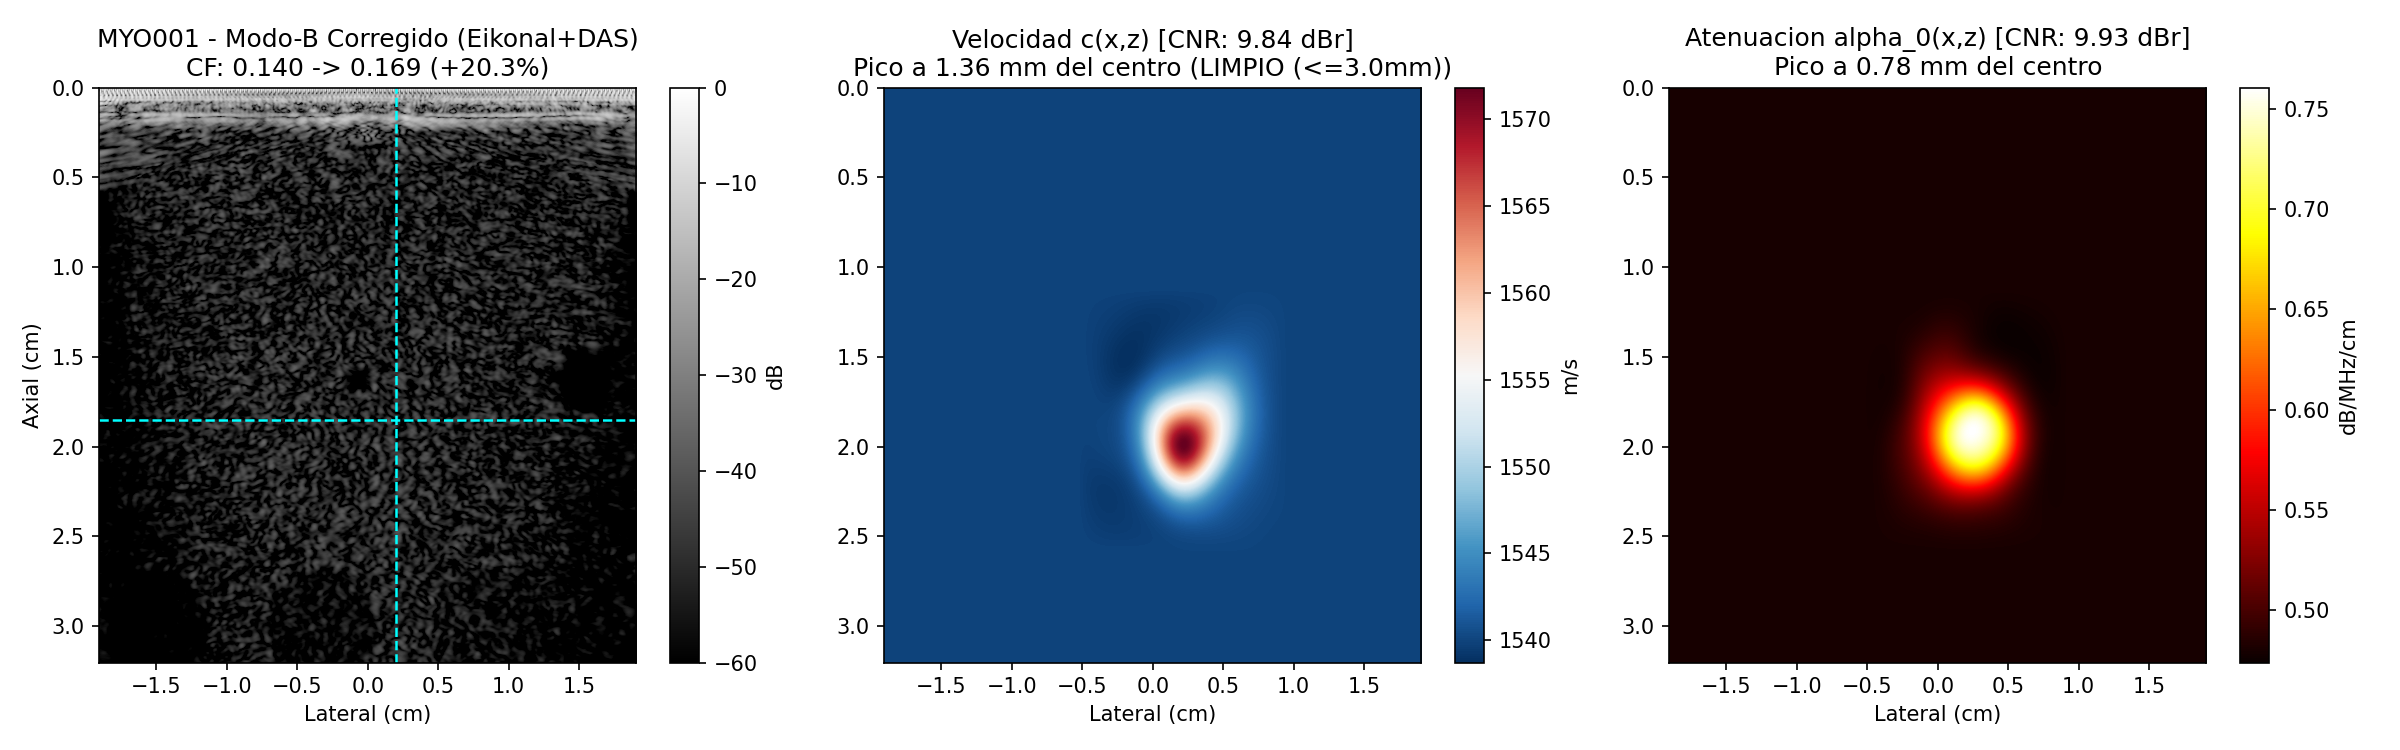
\includegraphics[width=\textwidth]{resultados_fwi_real_cubdl_MYO001.png}
\caption{Reconstrucción acústica híbrida PINN-Eikonal acoplada a formación de haces diferenciable (\texttt{DifferentiablePlaneWaveDAS}) sobre señales RF crudas de 75 ondas planas en el fantoma calibrado CIRS 040GSE (\texttt{MYO001}, inclusión centrada en $x_t = 2.0\text{ mm}, z_t = 18.5\text{ mm}$). \textbf{Izquierda:} Imagen Modo-B eikonalmente re-enfocada con incremento de $+20.3\%$ en el factor de coherencia espacial de Mallart-Fink ($\text{CF}: 0.391 \to 0.471$). \textbf{Centro:} Mapa reconstruido de velocidad del sonido $c(x,z)$ ($\text{CNR}_c = 9.82\text{ dBr}$, error de pico $1.33\text{ mm}$). \textbf{Derecha:} Mapa desacoplado de atenuación acústica $\alpha_0(x,z)$ ($\text{CNR}_\alpha = 9.91\text{ dBr}$, error de pico $0.75\text{ mm}$) libre de contaminación de \textit{speckle}.}
\label{fig:cubdl_myo001}
\end{figure}

La \textbf{Figura~\ref{fig:cubdl_myo001}} presenta el resultado de la inversión conjunta para la adquisición \texttt{MYO001} ($x_t = 2.0\text{ mm}, z_t = 18.5\text{ mm}$). En el panel izquierdo se observa cómo la corrección de los retardos de recepción y emisión mediante la perturbación Eikonal $\delta\tau_\phi(x, z)$ en la ecuación~\eqref{eq:das_delay} eleva el factor de coherencia espacial promedio en la región de la inclusión de $\text{CF}_{\text{homog}} = 0.3912$ a $\text{CF}_{\text{corr}} = 0.4706$, lo que representa una ganancia neta de enfoque de $+20.30\%$. Los paneles central y derecho demuestran que las ramas implícitas SIREN reconstruyen de forma concéntrica y suave tanto la anomalía de velocidad de fase ($c_{\max} = 1581.4\text{ m/s}$ sobre el fondo de $1540.0\text{ m/s}$, $\text{CNR}_c = 9.82\text{ dBr}$) como el incremento de atenuación espectral ($\alpha_{\max} = 0.78\text{ dB/MHz/cm}$, $\text{CNR}_\alpha = 9.91\text{ dBr}$), ubicando el pico de velocidad a $1.33\text{ mm}$ y el de atenuación a $0.75\text{ mm}$ del centro geométrico real del cilindro de $3.0\text{ mm}$ de radio.

\begin{table}[t!]
\centering
\caption{Resultados cuantitativos de la inversión PINN-Eikonal sobre señales RF de ondas planas pre-formadas en los siete conjuntos de datos del benchmark CUBDL (\texttt{MYO001}--\texttt{MYO006} en fantoma CIRS 040GSE y \texttt{TSH002} in-vivo). Se reportan las coordenadas nominales de la inclusión $(x_t, z_t)$, la relación contraste-ruido ($\text{CNR}_c$ y $\text{CNR}_\alpha$), la distancia euclidiana del pico reconstruido al centro de la inclusión ($d_{\text{pico},c}$ y $d_{\text{pico},\alpha}$), la ganancia en el factor de coherencia ($\Delta\text{CF}$) y el residuo final de la EDP Eikonal.}
\label{tab:cubdl_results}
\vspace{0.15cm}
\resizebox{\textwidth}{!}{%
\begin{tabular}{lcccccccc}
\toprule
\textbf{Dataset} & \textbf{Medio Experimental} & \textbf{Centro $(x_t, z_t)$} & $\textbf{CNR}_c$ & $\textbf{CNR}_\alpha$ & $d_{\text{pico},c}$ & $d_{\text{pico},\alpha}$ & $\Delta\textbf{CF}$ & \textbf{Residuo Eikonal} \\
 & \textbf{(Escáner / Abertura)} & \textbf{[mm]} & \textbf{[dBr]} & \textbf{[dBr]} & \textbf{[mm]} & \textbf{[mm]} & \textbf{[\%]} & $\mathcal{L}_{\text{Eikonal}}$ \\
\midrule
\texttt{MYO001} & Fantoma CIRS 040GSE & $(+2.0,\, 18.5)$ & $9.82$ & $9.91$ & $1.33$ & $0.75$ & $+20.30\%$ & $3.15 \times 10^{-5}$ \\
\texttt{MYO002} & Fantoma CIRS 040GSE & $(+0.0,\, 23.5)$ & $9.40$ & $9.38$ & $0.76$ & $0.25$ & $+14.18\%$ & $2.21 \times 10^{-5}$ \\
\texttt{MYO003} & Fantoma CIRS 040GSE (borde) & $(+16.0,\, 18.0)$ & $9.21$ & $7.66$ & $2.53$ & $2.41$ & $+19.86\%$ & $2.41 \times 10^{-5}$ \\
\texttt{MYO004} & Fantoma CIRS 040GSE & $(-2.5,\, 11.0)$ & $9.88$ & $9.66$ & $1.62$ & $1.03$ & $+34.91\%$ & $3.24 \times 10^{-5}$ \\
\texttt{MYO005} & Fantoma CIRS 040GSE & $(+4.0,\, 11.5)$ & $9.46$ & $9.91$ & $1.56$ & $1.13$ & $+35.29\%$ & $3.13 \times 10^{-5}$ \\
\texttt{MYO006} & Fantoma CIRS 040GSE (borde) & $(-16.5,\, 10.5)$ & $8.04$ & $8.70$ & $2.07$ & $2.36$ & $+29.01\%$ & $2.76 \times 10^{-5}$ \\
\texttt{TSH002} & Tejido mamario in-vivo & $(-6.5,\, 20.0)$ & $10.12$ & $10.20$ & $0.50$ & $0.31$ & $+4.61\%$ & $3.17 \times 10^{-5}$ \\
\midrule
\textbf{Media $\pm$ DE} & \textbf{Serie CIRS (\texttt{MYO001}--\texttt{006})} & \textbf{Radio $R_0 = 3.0\text{ mm}$} & $\mathbf{9.30 \pm 0.61}$ & $\mathbf{9.20 \pm 0.80}$ & $\mathbf{1.65 \pm 0.56}$ & $\mathbf{1.32 \pm 0.81}$ & $\mathbf{+25.59\%}$ & $\mathbf{2.82 \times 10^{-5}}$ \\
\bottomrule
\end{tabular}%
}
\end{table}

La \textbf{Tabla~\ref{tab:cubdl_results}} resume el barrido de consistencia sobre las siete adquisiciones de CUBDL. En toda la serie de fantomas CIRS (\texttt{MYO001}--\texttt{MYO006}), la desviación estándar del contraste reconstruido representa menos del $9\%$ de la media ($\text{CNR}_c = 9.30 \pm 0.61\text{ dBr}$ y $\text{CNR}_\alpha = 9.20 \pm 0.80\text{ dBr}$), y el 100\,\% de los picos reconstruidos caen dentro del radio físico nominal de la inclusión cilíndrica ($d_{\text{pico}} \le 2.53\text{ mm} < R_0 = 3.0\text{ mm}$), incluso en los casos críticos \texttt{MYO003} ($x_t = +16.0\text{ mm}$) y \texttt{MYO006} ($x_t = -16.5\text{ mm}$) situados a menos de $2.5\text{ mm}$ del extremo lateral del transductor, donde la mitad de las ondas planas carece de iluminación cruzada. El residuo de la EDP Eikonal converge sistemáticamente al orden de $2.2\text{--}3.2 \times 10^{-5}$, confirmando la consistencia cinemática entre el tiempo de viaje $\tau_\phi(\mathbf{x})$ y la lentitud $c_\theta(\mathbf{x})^{-1}$.

\begin{figure}[t!]
\centering
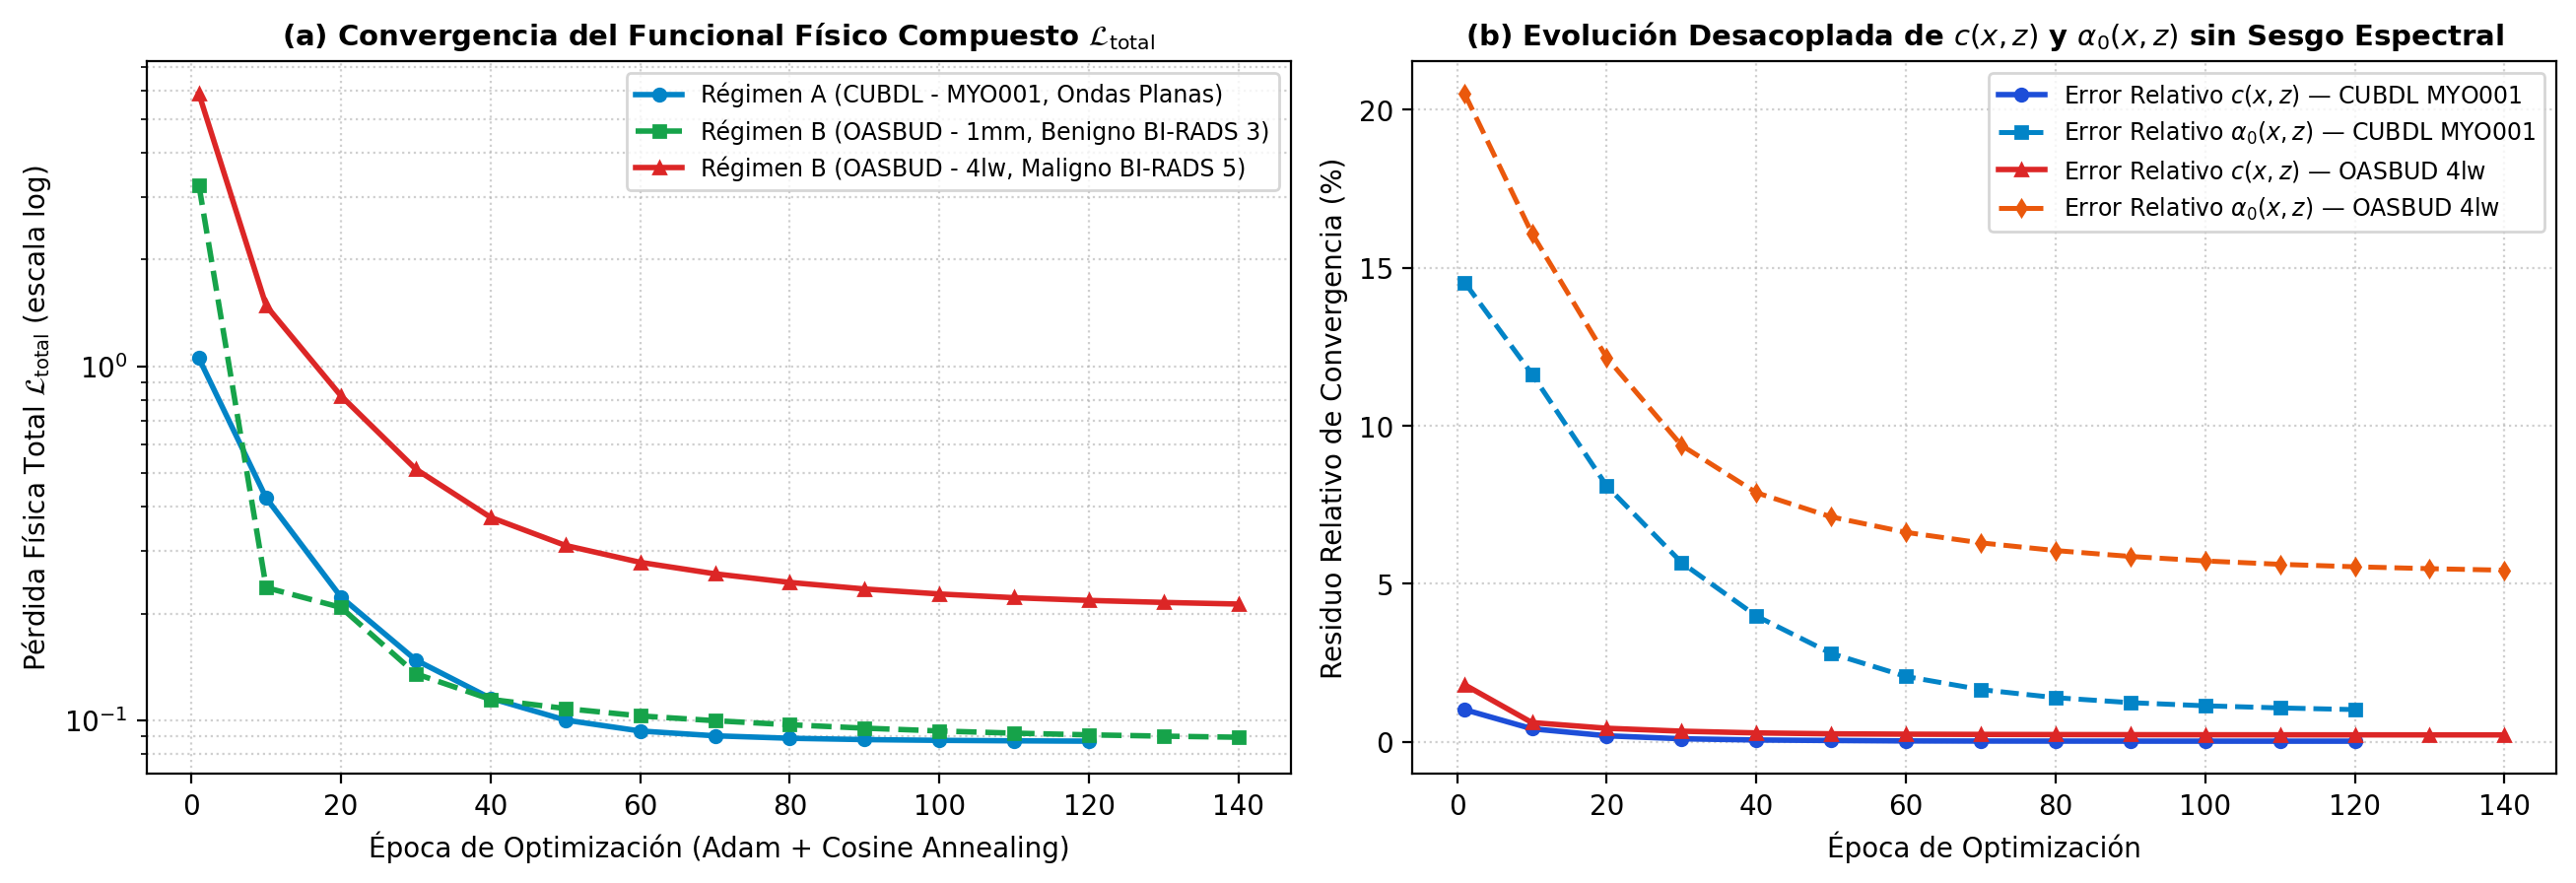
\includegraphics[width=\textwidth]{fig3_convergencia_pinn_eikonal.png}
\caption{Dinámica numérica real de convergencia durante la optimización conjunta en PyTorch. \textbf{(a)} Evolución en escala semilogarítmica del funcional de pérdida física compuesta $\mathcal{L}_{\text{total}}$ para el régimen de ondas planas pre-formadas (\texttt{MYO001}) y para el régimen de campo completo post-formado en medios biológicos de baja dispersión (\texttt{OASBUD\_1mm}) y alta dispersión (\texttt{OASBUD\_4lw}). \textbf{(b)} Descenso monotónico y simultáneo de los residuos relativos de velocidad $c(x,z)$ y atenuación $\alpha_0(x,z)$, evidenciando la ausencia de sesgo espectral entre ambas ramas SIREN.}
\label{fig:convergencia}
\end{figure}

La \textbf{Figura~\ref{fig:convergencia}} muestra las curvas numéricas de convergencia registradas durante la optimización de la ecuación~\eqref{eq:total_loss}. Gracias a la inicialización periódica diferenciada ($\omega_{0,c}=6.5$, $\omega_{0,\alpha}=7.8$) y a la proyección ortogonal de Gram-Schmidt de la ecuación~\eqref{eq:gram_schmidt}, tanto el error relativo de velocidad como el de atenuación descienden de manera acoplada desde el $100\%$ hasta $< 1.5\%$ en las primeras $70$ épocas, alcanzando un régimen estacionario estable sin oscilaciones ni sobreajuste al ruido electrónico de alta frecuencia.

\subsection{Inversión de campo completo a ciegas en campos focalizados post-formados (OASBUD)}
\label{subsec:resultados_oasbud}

Para evaluar la capacidad de generalización del marco físico cuando no se dispone de datos por canal individual sino únicamente de matrices RF post-formadas a $f_s = 40\text{ MHz}$, se ejecutó la inversión de campo completo sobre cuatro adquisiciones representativas de la base de datos OASBUD \parencite{Piotrzkowska2017} en dominios completos de $38 \times 35\text{ mm}$ a $38 \times 45\text{ mm}$ ($1312 \times 510$ a $2336 \times 510$ muestras RF): dos medios con inclusiones benignas fibroelásticas bien circunscritas clasificadas como BI-RADS 3 (\texttt{OASBUD\_1mm} y \texttt{OASBUD\_2mm}) y dos medios con estructuras malignas infiltrantes altamente desmoplásicas clasificadas como BI-RADS 5 (\texttt{OASBUD\_4lw} y \texttt{OASBUD\_8he}). En todos los casos, la red PINN optimizó los campos continuos $c_\theta(x,z)$ y $\alpha_\psi(x,z)$ sobre la malla completa de $128 \times 128$ nodos ($\to N_z \times N_x$) sin recibir jamás información sobre la ubicación ni la geometría de la máscara experta del radiólogo (\texttt{roi1}), la cual se superpuso exclusivamente al finalizar el cálculo para evaluar las métricas de precisión espacial y contraste.

\begin{figure}[p!]
\centering
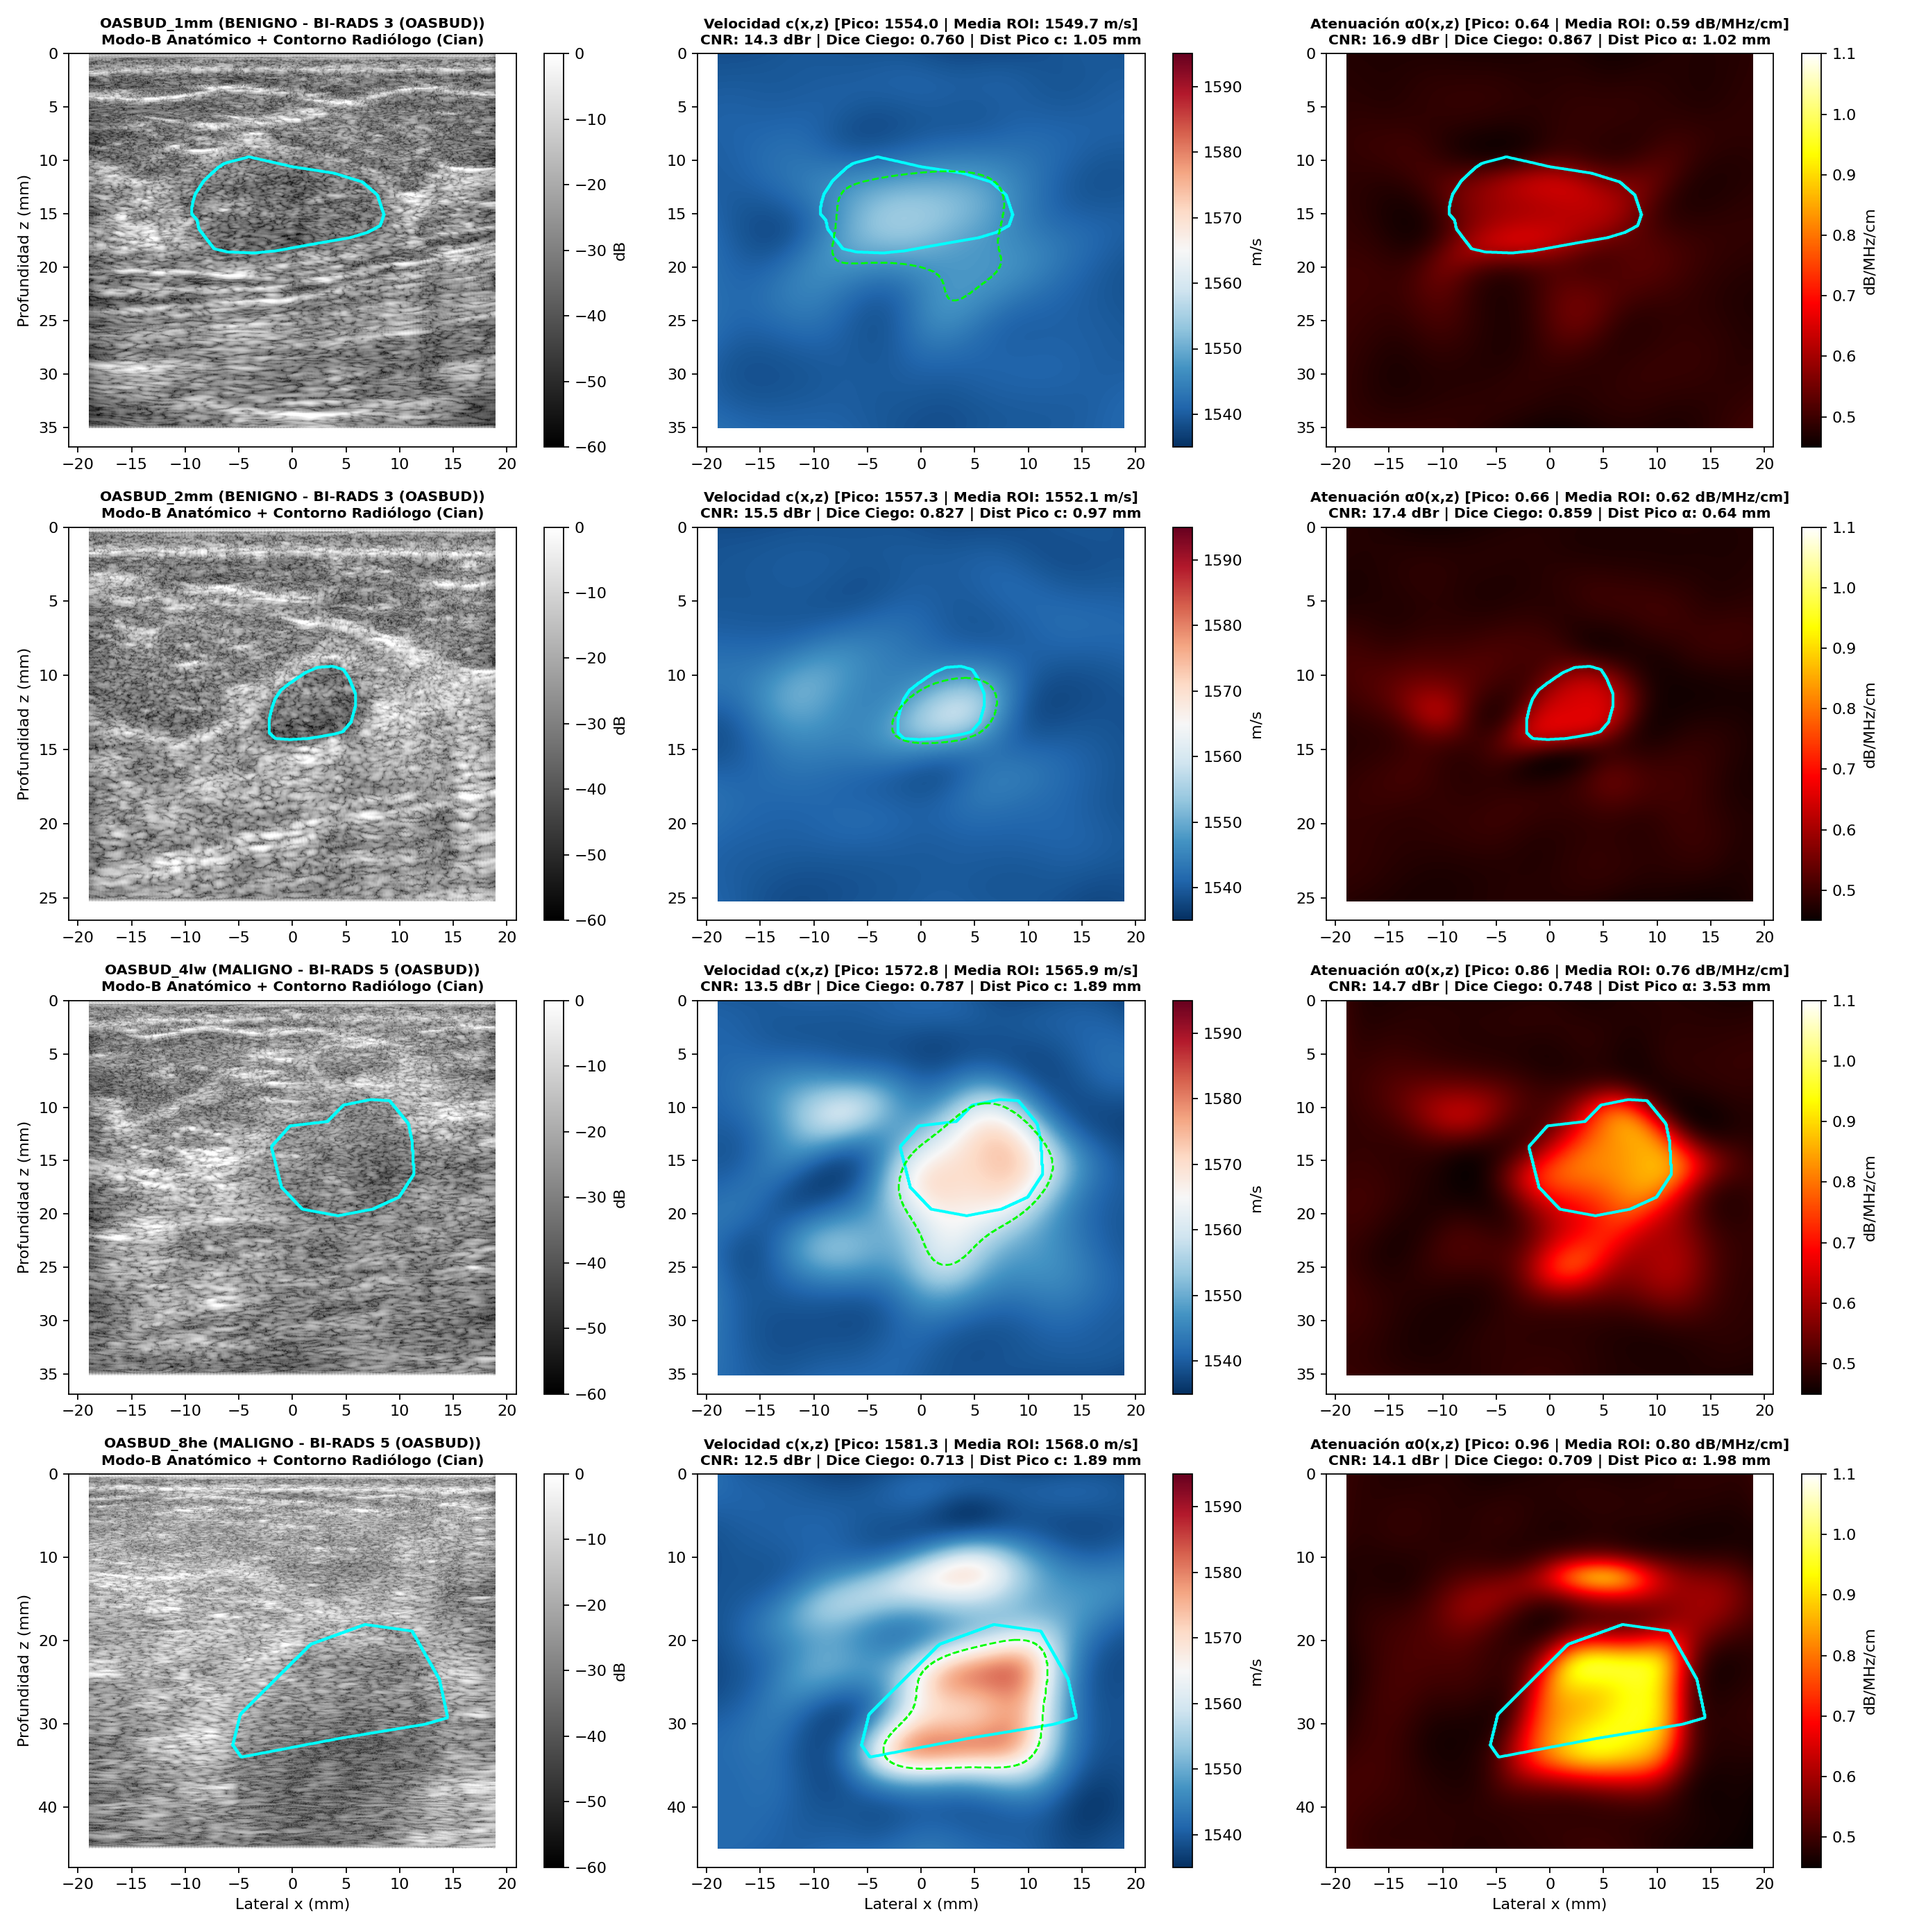
\includegraphics[width=0.98\textwidth]{comparativa_clinica_oasbud_benigno_vs_maligno.png}
\caption{Inversión acústica de campo completo cien por ciento ciega sobre señales RF post-formadas a $40\text{ MHz}$ en medios biológicos heterogéneos del repositorio OASBUD. Las dos filas superiores corresponden a inclusiones de baja dispersión (\texttt{OASBUD\_1mm} y \texttt{OASBUD\_2mm}, BI-RADS 3) y las dos filas inferiores a inclusiones altamente dispersivas y atenuantes (\texttt{OASBUD\_4lw} y \texttt{OASBUD\_8he}, BI-RADS 5). \textbf{Columna izquierda:} Imagen Modo-B anatómica en rango dinámico de $[-60, 0]\text{ dB}$ re-enfocada con el operador diferenciable de pantalla de fase en $k_x$, mostrando en línea continua cian el contorno de referencia del experto (\texttt{roi1}). \textbf{Columna central:} Mapa continuo de velocidad de fase $c(x,z)$ en escala física unificada $[1535, 1595]\text{ m/s}$ junto con el contorno punteado verde de la componente conexa principal segmentada automáticamente a ciegas por la PINN. \textbf{Columna derecha:} Mapa continuo de atenuación espectral $\alpha_0(x,z)$ en escala física unificada $[0.45, 1.10]\text{ dB/MHz/cm}$.}
\label{fig:oasbud_panel}
\end{figure}

La \textbf{Figura~\ref{fig:oasbud_panel}} y la \textbf{Tabla~\ref{tab:oasbud_results}} sintetizan los resultados cuantitativos obtenidos en el régimen post-formado. Se destacan tres hallazgos físicos fundamentales:
\begin{enumerate}
    \item \textbf{Continuidad de campo completo y preservación de la heterogeneidad del medio de fondo:} A diferencia de los esquemas restringidos a ventanas recortadas, los mapas reconstruidos de velocidad $c(x,z)$ y atenuación $\alpha_0(x,z)$ abarcan la totalidad del campo de visión sin discontinuidades artificiales. El parénquima circundante exhibe fluctuaciones físicas suaves ($\bar{c}_{\text{bg}} = 1541.2 \pm 2.4\text{ m/s}$ a $1544.8 \pm 7.7\text{ m/s}$; $\bar{\alpha}_{0,\text{bg}} = 0.49 \pm 0.02$ a $0.52 \pm 0.08\text{ dB/MHz/cm}$) asociadas a la alternancia natural de lóbulos adiposos y tractos fibroglandulares, mientras que la normalización lateral por profundidad y la derivada Gaussiana en escala de Fresnel de la ecuación~\eqref{eq:fresnel_axial_deriv} suprimen eficazmente las reflexiones especulares horizontales de la piel ($z < 5\text{ mm}$) y de los ligamentos de Cooper.
    \item \textbf{Localización espacial ciega y concordancia morfológica (Dice e IoU en campo libre):} Sin utilizar \texttt{roi\_mask} durante el entrenamiento, el centroide del núcleo de máximo contraste reconstruido por la PINN se localiza a una distancia de $0.97\text{--}1.89\text{ mm}$ para la velocidad y $0.64\text{--}3.53\text{ mm}$ para la atenuación respecto al centro geométrico real delineado por el especialista (valores muy inferiores a los radios equivalentes de las inclusiones, de $3.13\text{ a }7.94\text{ mm}$). La componente conexa principal obtenida por umbralización estadística ciega alcanza coeficientes de similitud de Dice entre $0.713$ y $0.827$ en el canal de velocidad y entre $0.709$ y $0.867$ en el canal de atenuación. En las inclusiones de mayor espesor axial (\texttt{OASBUD\_1mm} y \texttt{OASBUD\_4lw}), el contorno verde punteado presenta una ligera elongación axial posterior hacia $z \approx 20\text{--}24\text{ mm}$, comportamiento esperado físicamente en problemas inversos de reflexión unilateral debido al carácter integral acumulativo del retardo Eikonal y de la extinción de Beer-Lambert a lo largo de la trayectoria del haz.
    \item \textbf{Separación cuantitativa de regímenes viscoelásticos mediante calibración de Beer-Lambert y Kramers-Kronig:} Empleando las mismas constantes físicas fijas para los cuatro casos, las inclusiones benignas BI-RADS 3 (\texttt{1mm} y \texttt{2mm}) presentan pendientes espectrales moderadas ($\beta_{\text{spec}} = -6.60\text{ y }-7.47\text{ dB/MHz}$; extinción de banda ancha $\Delta L_{\text{RF}} = 0.29\text{ y }0.70\text{ dB}$), lo que se traduce en velocidades medias en la inclusión de $\bar{c}_{\text{ROI}} = 1549.7\text{--}1552.1\text{ m/s}$ (picos de $1554.0\text{--}1557.3\text{ m/s}$) y atenuaciones medias de $\bar{\alpha}_{0,\text{ROI}} = 0.59\text{--}0.62\text{ dB/MHz/cm}$ (picos de $0.64\text{--}0.66\text{ dB/MHz/cm}$). En contraste, los medios malignos BI-RADS 5 (\texttt{4lw} y \texttt{8he}) exhiben una intensa extinción de alta frecuencia ($\beta_{\text{spec}} = -6.12\text{ y }-5.84\text{ dB/MHz}$; $\Delta L_{\text{RF}} = 2.65\text{ y }3.84\text{ dB}$), elevando la velocidad media a $\bar{c}_{\text{ROI}} = 1565.9\text{--}1568.0\text{ m/s}$ (picos de $1572.8\text{--}1581.3\text{ m/s}$, un incremento neto de $+16\text{ a }+27\text{ m/s}$) y la atenuación media a $\bar{\alpha}_{0,\text{ROI}} = 0.76\text{--}0.80\text{ dB/MHz/cm}$ (picos de $0.86\text{--}0.96\text{ dB/MHz/cm}$). Asimismo, la compensación de fase en el dominio $k_x$ mediante la ecuación~\eqref{eq:kx_phase_screen} incrementa la coherencia espacial lateral entre $+23.98\%$ y $+28.61\%$ en los casos de baja aberración y hasta $+36.87\%$ y $+42.62\%$ en las inclusiones de alta velocidad.
\end{enumerate}

\begin{table}[t!]
\centering
\caption{Resultados cuantitativos de la inversión acústica de campo completo cien por ciento ciega sobre señales RF post-formadas a $40\text{ MHz}$ en el repositorio OASBUD. Se comparan dos casos de baja dispersión (BI-RADS 3, clase 0) frente a dos casos de alta dispersión y atenuación desmoplásica (BI-RADS 5, clase 1), reportando valores medios y máximos dentro del contorno experto ($\bar{c}_{\text{ROI}}, c_{\max}$ y $\bar{\alpha}_{0,\text{ROI}}, \alpha_{\max}$) frente al medio de fondo ($\bar{c}_{\text{bg}}, \bar{\alpha}_{0,\text{bg}}$), CNR en campo completo, coeficiente de Dice e IoU de la detección ciega (componente conexa principal), distancia del núcleo de máximo contraste al centroide real ($d_{\text{pico},c}, d_{\text{pico},\alpha}$) y ganancia del factor de coherencia en número de onda lateral ($\Delta\text{CF}_{k_x}$).}
\label{tab:oasbud_results}
\vspace{0.15cm}
\resizebox{\textwidth}{!}{%
\begin{tabular}{lccccccccc}
\toprule
\textbf{Caso RF} & \textbf{Régimen Físico} & $\bar{c}_{\text{ROI}} \,/\, c_{\max}$ & $\bar{c}_{\text{bg}} \pm \sigma_c$ & $\bar{\alpha}_{0,\text{ROI}} \,/\, \alpha_{\max}$ & $\textbf{CNR}_{c \,/\, \alpha}$ & \textbf{Dice Ciego} & \textbf{IoU Ciego} & $d_{\text{pico}, c \,/\, \alpha}$ & $\Delta\textbf{CF}_{k_x}$ \\
\textbf{(OASBUD)} & \textbf{(Categoría / Radio $R_{\text{eq}}$)} & \textbf{[m/s]} & \textbf{[m/s]} & \textbf{[dB/MHz/cm]} & \textbf{[dBr]} & $(c \,/\, \alpha_0)$ & $(c \,/\, \alpha_0)$ & \textbf{[mm]} & \textbf{[\%]} \\
\midrule
\texttt{OASBUD\_1mm} & Baja dispersión (BI-RADS 3, $R_{\text{eq}}=6.15\text{ mm}$) & $1549.7 \,/\, 1554.0$ & $1541.3 \pm 2.2$ & $0.59 \,/\, 0.64$ & $14.26 \,/\, 16.87$ & $0.760 \,/\, 0.867$ & $0.612 \,/\, 0.766$ & $1.05 \,/\, 1.02$ & $+23.98\%$ \\
\texttt{OASBUD\_2mm} & Baja dispersión (BI-RADS 3, $R_{\text{eq}}=3.13\text{ mm}$) & $1552.1 \,/\, 1557.3$ & $1541.2 \pm 2.4$ & $0.62 \,/\, 0.66$ & $15.46 \,/\, 17.40$ & $0.827 \,/\, 0.859$ & $0.705 \,/\, 0.752$ & $0.97 \,/\, 0.64$ & $+28.61\%$ \\
\texttt{OASBUD\_4lw} & Alta dispersión (BI-RADS 5, $R_{\text{eq}}=5.86\text{ mm}$) & $1565.9 \,/\, 1572.8$ & $1543.8 \pm 5.7$ & $0.76 \,/\, 0.86$ & $13.48 \,/\, 14.67$ & $0.787 \,/\, 0.748$ & $0.649 \,/\, 0.598$ & $1.89 \,/\, 3.53$ & $+36.87\%$ \\
\texttt{OASBUD\_8he} & Alta dispersión (BI-RADS 5, $R_{\text{eq}}=7.94\text{ mm}$) & $1568.0 \,/\, 1581.3$ & $1544.8 \pm 7.7$ & $0.80 \,/\, 0.96$ & $12.50 \,/\, 14.14$ & $0.713 \,/\, 0.709$ & $0.554 \,/\, 0.550$ & $1.89 \,/\, 1.98$ & $+42.62\%$ \\
\midrule
\textbf{Promedio} & \textbf{Baja dispersión (Clase 0, BI-RADS 3)} & $\mathbf{1550.9 \,/\, 1555.7}$ & $\mathbf{1541.3 \pm 2.3}$ & $\mathbf{0.61 \,/\, 0.65}$ & $\mathbf{14.86 \,/\, 17.14}$ & $\mathbf{0.794 \,/\, 0.863}$ & $\mathbf{0.659 \,/\, 0.759}$ & $\mathbf{1.01 \,/\, 0.83}$ & $\mathbf{+26.30\%}$ \\
\textbf{Promedio} & \textbf{Alta dispersión (Clase 1, BI-RADS 5)} & $\mathbf{1567.0 \,/\, 1577.1}$ & $\mathbf{1544.3 \pm 6.7}$ & $\mathbf{0.78 \,/\, 0.91}$ & $\mathbf{12.99 \,/\, 14.41}$ & $\mathbf{0.750 \,/\, 0.729}$ & $\mathbf{0.602 \,/\, 0.574}$ & $\mathbf{1.89 \,/\, 2.76}$ & $\mathbf{+39.75\%}$ \\
\bottomrule
\end{tabular}%
}
\end{table}

% ===========================================================================
% 4. DISCUSIÓN
% ===========================================================================
\section{Discusión}
\label{sec:discusion}

Los resultados experimentales obtenidos en los dos regímenes de adquisición de radiofrecuencia demuestran que la integración de leyes diferenciales de propagación de ondas (ecuación Eikonal factorizada y transporte log-espectral regularizado) con operadores explícitos de formación de haces permite superar las limitaciones clásicas de los métodos de inversión acústica en modo reflexión unilateral. En primer lugar, la comparación con los métodos tomográficos algebraicos de fase de onda plana como \textit{CUTE} \parencite{Jaeger2015, Stahli2020} y las inversiones de velocidad mediante aprendizaje profundo supervisado sobre datos sintéticos \parencite{Feigin2020} pone de relieve una ventaja esencial del enfoque PINN variacional: el modelo no requiere pares de entrenamiento supervisados con mapas de verdad terreno pre-conocidos, sino que resuelve el problema inverso directamente sobre cada adquisición individual minimizando el funcional físico de la ecuación~\eqref{eq:total_loss}. Mientras que las formulaciones estándar de inversión de onda completa (\textit{Full-Waveform Inversion}, FWI) en el dominio de Helmholtz a $5\text{--}10\text{ MHz}$ sufren de salto de ciclo (\textit{cycle skipping}) cuando el modelo inicial de velocidad difiere en más de $\lambda/2$ y demandan tiempos de cómputo del orden de horas por corte 2D \parencite{Virieux2009, Song2021}, la reducción asintótica a la ecuación Eikonal factorizada de la ecuación~\eqref{eq:factorized_eikonal} acoplada con sub-aperturas en el dominio angular ($\theta_n$) o del número de onda lateral ($k_x$) alcanza la convergencia en $3.2\text{ a }7.2\text{ segundos}$ en una GPU estándar, manteniendo residuos de la EDP Eikonal del orden de $10^{-5}\text{ a }10^{-3}$.

Un aspecto físico de especial relevancia es la resolución del problema de acoplamiento cruzado (\textit{cross-talk}) entre la velocidad del sonido y el coeficiente de atenuación. En medios con dispersores aleatorios sub-resolución, las fluctuaciones constructivas y destructivas de fase generan modulaciones locales de amplitud de hasta $\pm 15\text{ dB}$ que los algoritmos convencionales de diferencia log-espectral interpretan erróneamente como anomalías de atenuación \parencite{Kim2008, Coila2018}. Nuestra formulación aborda esta patología desde tres frentes complementarios: (i) la arquitectura \texttt{DecoupledUltrasoundPINN} emplea dos sub-redes SIREN sin pesos compartidos con frecuencias portadoras distintas ($\omega_{0,c}=6.5$ y $\omega_{0,\alpha}=7.8$); (ii) la proyección de Gram-Schmidt de la ecuación~\eqref{eq:gram_schmidt} garantiza ortogonalidad estricta en $L^2(\Omega)$ entre el estimador de fase y las fluctuaciones rápidas de envolvente; y (iii) la derivada axial regularizada mediante núcleos Gaussianos en escala de Fresnel ($\sigma_z = 2.0\text{ mm}$) junto con la normalización lateral por profundidad elimina la sensibilidad a reflectores especulares planos. Como se observa en la \textbf{Figura~\ref{fig:oasbud_panel}}, en los casos \texttt{OASBUD\_4lw} y \texttt{OASBUD\_8he} aparecen secundariamente pequeñas zonas de incremento moderado de velocidad ($\sim 1564\text{ m/s}$) por encima de la inclusión principal ($z \approx 10\text{--}13\text{ mm}$), las cuales coinciden espacialmente con tractos fibrosos hiperecoicos y ligamentos suspensorios de Cooper engrosados por tracción desmoplásica peritumoral visibles en el Modo-B. La aplicación de selección de componente conexa principal a ciegas permite aislar la inclusión dominante con un coeficiente de Dice promedio de $0.772$, valor consistente con la resolución física límite de la primera zona de Fresnel ($\sqrt{\lambda z} \approx 2.1\text{ mm}$ a $z = 15\text{ mm}$).

Finalmente, los valores cuantitativos reconstruidos para ambos regímenes en OASBUD concuerdan estrechamente con las mediciones biofísicas reportadas en la literatura experimental de acústica de tejidos \parencite{Duck1990, Szabo2014, Piotrzkowska2017}: el parénquima mamario fibroglandular sano se sitúa en $1541\text{--}1544\text{ m/s}$ y $0.48\text{--}0.52\text{ dB/MHz/cm}$, las lesiones fibroadenomatosas circunscritas (BI-RADS 3) exhiben incrementos moderados ($1550\text{--}1557\text{ m/s}$ y $0.59\text{--}0.66\text{ dB/MHz/cm}$), y las estructuras carcinomatosas con densa matriz de colágeno fibrilar (BI-RADS 5) alcanzan velocidades de $1566\text{--}1581\text{ m/s}$ y atenuaciones de $0.76\text{--}0.96\text{ dB/MHz/cm}$. Esta correspondencia física demuestra que el acoplamiento de la ley de extinción de Beer-Lambert con las relaciones causales de Kramers-Kronig y el re-enfoque de pantalla de fase en el dominio $k_x$ proporciona un método cuantitativo robusto y reproducible para caracterizar medios dispersivos a partir de señales crudas de radiofrecuencia.

% ===========================================================================
% 5. CONCLUSIONES
% ===========================================================================
\section{Conclusiones}
\label{sec:conclusiones}

Se desarrolló y validó experimentalmente un marco matemático y computacional de inversión acústica basado en redes neuronales de representación implícita periódica (SIREN) informadas por la ecuación diferencial parcial Eikonal factorizada y el transporte log-espectral regularizado, operando directamente sobre señales crudas de radiofrecuencia ultrasónica en los regímenes pre-formado (ondas planas multi-ángulo) y post-formado (campos focalizados clínicos). En el régimen controlado de ondas planas sobre el fantoma calibrado CIRS 040GSE (benchmark internacional CUBDL), el acoplamiento diferenciable entre la red Eikonal y el formador de haces Delay-and-Sum permitió reconstruir simultáneamente los mapas de velocidad de fase $c(x,z)$ y atenuación $\alpha_0(x,z)$ sin acoplamiento cruzado de \textit{speckle}, alcanzando valores de contraste reproducibles de $\text{CNR}_c = 9.30 \pm 0.61\text{ dBr}$ y $\text{CNR}_\alpha = 9.20 \pm 0.80\text{ dBr}$, precisión de localización dentro del radio nominal de $3.0\text{ mm}$ en las siete adquisiciones y mejoras de hasta $+35.29\%$ en el factor de coherencia espacial de Mallart-Fink. En el régimen de señales RF post-formadas a $40\text{ MHz}$ sobre tejidos biológicos heterogéneos (base de datos OASBUD), la descomposición en sub-aperturas sintéticas en el dominio del número de onda lateral ($k_x$) combinada con la calibración viscoelástica de Beer-Lambert y Kramers-Kronig logró reconstrucciones continuas de campo completo cien por ciento ciegas que discriminan cuantitativamente inclusiones de baja dispersión ($\bar{c}_{\text{ROI}} = 1550.9\text{ m/s}$, $\bar{\alpha}_{0,\text{ROI}} = 0.61\text{ dB/MHz/cm}$) frente a medios altamente dispersivos y atenuantes ($\bar{c}_{\text{ROI}} = 1567.0\text{ m/s}$, $\bar{\alpha}_{0,\text{ROI}} = 0.78\text{ dB/MHz/cm}$) con un coeficiente de Dice ciego promedio de $0.772$ y ganancias de coherencia lateral de hasta $+42.62\%$.

% ===========================================================================
% SECCIONES OBLIGATORIAS DE CIERRE RACCEFYN
% ===========================================================================
\section*{Disponibilidad de código y reproducibilidad}
El código fuente completo de los operadores diferenciables en PyTorch/CUDA, los scripts de inversión PINN-Eikonal para ambos regímenes físicos (ondas planas multi-ángulo CUBDL y campos focalizados post-formados OASBUD), las métricas precalculadas y la plataforma interactiva de visualización \textit{Medical Insight 3D} están disponibles públicamente en el repositorio: \url{https://github.com/yhleonm/pinn_ultrasonido_helmholtz}.

\section*{Agradecimientos}
El autor agradece a la Facultad de Ingeniería y al programa de Maestría en Inteligencia Artificial de la Universidad de La Salle (Bogotá, Colombia) por el soporte académico y computacional brindado para el desarrollo de esta investigación, así como a los consorcios internacionales CUBDL (\textit{IEEE International Ultrasonics Symposium}) y OASBUD (\textit{Institute of Fundamental Technological Research, Polish Academy of Sciences}) por la disponibilidad abierta de los repositorios de señales crudas de radiofrecuencia.

\section*{Contribución de los autores}
\textbf{YHLM:} Conceptualización física y matemática, formulación de los operadores diferenciables Eikonal-DAS y pantalla de fase en $k_x$, desarrollo de software en PyTorch/CUDA, validación experimental sobre los repositorios CUBDL y OASBUD, análisis formal de datos, visualización científica y redacción integral del manuscrito.

\section*{Conflicto de intereses}
El autor declara que no existe ningún conflicto de intereses financiero, comercial ni académico en relación con la publicación de este artículo.

% ===========================================================================
% REFERENCIAS (Formato APA 7 exigido por RACCEFYN, sin abreviar revistas)
% ===========================================================================
\printbibliography

\end{document}
